% บทที่ 3 วิธีดำเนินการและการออกแบบระบบ
% สร้างจาก Google Doc "Collab_Reflect_Report" — แก้เนื้อหาในไฟล์นี้ได้โดยตรง
% ต้องมี: \usepackage{graphicx} (template มีแล้ว) และ xltabular (cpecmu.cls โหลดให้แล้ว)
% คอลัมน์ Y และ P ประกาศไว้ในไฟล์หลัก (sampleReport.tex) เพื่อใช้ร่วมกับบทที่ 2

\chapter{วิธีดำเนินการและการออกแบบระบบ}
\label{ch:method}

ในบทนี้จะกล่าวถึงขั้นตอนการดำเนินงานของโครงงาน ตั้งแต่การสำรวจบริบทของปัญหา การเก็บข้อมูลความต้องการจากอาจารย์ผู้สอน การแปลงความต้องการเป็นฟีเจอร์ของระบบ การออกแบบเกณฑ์การประเมิน หลักการทำงานของระบบ การออกแบบส่วนปัญญาประดิษฐ์ (AI) สถาปัตยกรรมและฐานข้อมูล ส่วนต่อประสานผู้ใช้ ความปลอดภัยและการคุ้มครองข้อมูลส่วนบุคคล ไปจนถึงแผนการประเมินระบบและตัวชี้วัดความสำเร็จ

\section{ภาพรวมวิธีดำเนินงาน}\label{sec:3.1}

ระบบนิเวศการเรียนรู้ประกอบด้วยผู้เรียน ผู้สอน กระบวนการเรียนการสอน เป้าหมายการเรียนรู้ และกระบวนการให้ข้อเสนอแนะ เป้าหมายการเรียนรู้มีทั้งทักษะเฉพาะทาง (hard skill) และทักษะด้านอื่น (soft skill) โครงงานนี้ไม่ได้มุ่งแก้ปัญหาทุกส่วนของระบบนิเวศดังกล่าว แต่เลือกโฟกัสที่ทักษะการทำงานเป็นทีม (teamwork) ซึ่งเป็น soft skill ที่อาจารย์สังเกตได้ยากที่สุดในรายวิชาขนาดใหญ่ และกระบวนการให้ข้อเสนอแนะระหว่างเพื่อนในทีม (peer feedback) ที่ช่วยให้ผู้เรียนพัฒนาทักษะนั้น การดำเนินงานแบ่งออกเป็น 4 ระยะ ดังตารางที่~\ref{tab:ch3-1}

\begin{xltabular}{\textwidth}{|P{0.17\textwidth}|Y|P{0.2\textwidth}|P{0.2\textwidth}|}
\caption{กิจกรรม ผลลัพธ์ และสถานะของแต่ละระยะ}\label{tab:ch3-1}\\
\hline \textbf{ระยะ} & \textbf{กิจกรรมหลัก} & \textbf{ผลลัพธ์} & \textbf{ช่วงเวลาและสถานะ} \\ \hline
\endfirsthead
\multicolumn{4}{r}{\small (ต่อ)}\\ \hline \textbf{ระยะ} & \textbf{กิจกรรมหลัก} & \textbf{ผลลัพธ์} & \textbf{ช่วงเวลาและสถานะ} \\ \hline
\endhead
1. สำรวจบริบทของปัญหา & ทบทวนงานวิจัยด้านการทำงานเป็นทีม การประเมินเพื่อนร่วมทีม และข้อเสนอแนะเชิงสร้างสรรค์ ศึกษาระบบที่มีอยู่ ได้แก่ CATME, FeedbackFruits และ Peerceptiv & ขอบเขตของปัญหาและตารางเปรียบเทียบระบบที่มีอยู่ & ก.ค.--ส.ค. 2569 (เสร็จแล้ว) \\ \hline
2. เก็บข้อมูลความต้องการ & สัมภาษณ์อาจารย์ผู้สอน 5 ท่าน ทั้งในและนอกภาควิชา & ปัญหา ความต้องการ และความคาดหวังของผู้ใช้ & ก.ย. 2569 (เสร็จแล้ว) \\ \hline
3. ออกแบบและทดลอง & แบ่งฟีเจอร์เป็นช่วงออกแบบเกณฑ์ประเมิน ขั้นตอนการทำงาน ฐานข้อมูล และต้นแบบหน้าจอ (wireframe) & เอกสารการออกแบบและต้นแบบหน้าจอ & ส.ค. 2569--ปัจจุบัน (กำลังดำเนินการ เริ่มพัฒนาระยะที่ 1) \\ \hline
4. ตรวจสอบและใช้งานจริง & ทดสอบระบบ นำร่องใช้ในรายวิชาจริง และเก็บผลตอบรับจากผู้ใช้ & ผลการประเมินระบบตามตัวชี้วัด & ภาคการศึกษาที่ 2 ปีการศึกษา 2569 (ยังไม่เริ่ม) \\ \hline
\end{xltabular}

ณ วันที่จัดทำรายงานฉบับนี้ โครงงานดำเนินงานระยะที่ 1 และ 2 เสร็จสิ้นแล้ว และอยู่ในระยะที่ 3 โดยออกแบบระบบเสร็จแล้วและกำลังเริ่มพัฒนาเว็บแอปพลิเคชันในระยะที่ 1

\section{การเก็บข้อมูลความต้องการ}\label{sec:3.2}

\subsection{ผู้ให้ข้อมูลและวิธีการ}\label{sec:3.2.1}

คณะผู้จัดทำสัมภาษณ์อาจารย์ผู้สอนรายวิชาที่มีการทำงานกลุ่มจำนวน 5 ท่าน แบ่งเป็น 2 กลุ่ม ได้แก่ อาจารย์ภาควิชาวิศวกรรมคอมพิวเตอร์ 3 ท่าน เพื่อศึกษาปัญหาในบริบทที่เป็นจุดเริ่มต้นของโครงงาน และอาจารย์ภาควิชาวิศวกรรมอุตสาหการ 2 ท่าน เพื่อศึกษามุมมองจากบริบทการสอนที่แตกต่างกัน การสัมภาษณ์เป็นแบบกึ่งโครงสร้าง (semi-structured interview) ครอบคลุม 6 ประเด็น ได้แก่

\begin{itemize}
  \item ปัญหาการทำงานกลุ่ม
  \item เป้าหมายของการประเมินเพื่อน (peer review)
  \item รูปแบบคะแนนและฟีดแบ็ก
  \item การประยุกต์ใช้ปัญญาประดิษฐ์ (AI)
  \item การเชื่อมต่อกับระบบอื่น
  \item ความต้องการและข้อจำกัดของระบบ
\end{itemize}

รายการคำถามที่ใช้ในการสัมภาษณ์แสดงไว้ในภาคผนวก ก จากนั้นคณะผู้จัดทำนำคำตอบมาจัดกลุ่มเป็น 3 หมวด คือ ปัญหาที่พบ (pain point) ความต้องการต่อระบบ (needs) และความคาดหวังต่อบทบาทของระบบ (expectations) แล้วเปรียบเทียบประเด็นที่อาจารย์เห็นตรงกันและเห็นต่างกัน

\subsection{ผลการสัมภาษณ์}\label{sec:3.2.2}

ผลการสัมภาษณ์สรุปตามหมวดได้ดังตารางที่~\ref{tab:ch3-2}

\begin{xltabular}{\textwidth}{|P{0.22\textwidth}|Y|}
\caption{สรุปผลการสัมภาษณ์อาจารย์ผู้สอน 5 ท่าน}\label{tab:ch3-2}\\
\hline \textbf{หมวด} & \textbf{ประเด็นที่พบ} \\ \hline
\endfirsthead
\multicolumn{2}{r}{\small (ต่อ)}\\ \hline \textbf{หมวด} & \textbf{ประเด็นที่พบ} \\ \hline
\endhead
ปัญหาที่พบ (pain point) & (1) อาจารย์มองไม่เห็นพฤติกรรมการทำงานของนักศึกษานอกห้องเรียน (2) เกิดภาวะสมาชิกไม่ช่วยงาน (free-rider) และสมาชิกที่ต้องแบกงาน (3) การสื่อสารภายในทีมคลาดเคลื่อน (4) ข้อเสนอแนะระหว่างเพื่อนมักใช้อารมณ์หรือไม่สร้างสรรค์ (5) ขาดเครื่องมือเก็บข้อมูลเชิงประจักษ์เพื่อวัดผล soft skill \\ \hline
ความต้องการต่อระบบ (needs) & (1) ระบบเรียบง่ายและไม่เพิ่มภาระอาจารย์ (2) เชื่อมต่อกับ Mango Canvas เพื่อลดการกรอกข้อมูลซ้ำ (3) เริ่มจากการประเมินระดับชิ้นงาน (assignment) ที่เรียบง่ายและเสถียรก่อน (4) เกณฑ์ชัดเจนและหน้าจออ่านง่าย (5) ให้ความสำคัญกับความเป็นส่วนตัวของข้อมูล \\ \hline
ความคาดหวังต่อบทบาทของระบบ (expectations) & (1) การประเมินเพื่อนไม่ใช่เพียงเครื่องมือตัดเกรด แต่เป็นพื้นที่สะท้อนพฤติกรรมและการมีส่วนร่วม (2) มุ่งเน้นข้อเสนอแนะเชิงสร้างสรรค์เพื่อการพัฒนาตนเอง ด้วยภาษาที่นุ่มนวล (3) ช่วยให้นักศึกษาเข้าใจบทบาท ความรับผิดชอบ และพลวัตภายในทีม \\ \hline
\end{xltabular}

\subsection{ประเด็นที่เห็นต่างและการตัดสินใจออกแบบ}\label{sec:3.2.3}

อาจารย์ทุกท่านเห็นตรงกันว่าระบบต้องเรียบง่าย เชื่อมต่อกับระบบของมหาวิทยาลัยเพื่อลดภาระ และเน้นข้อเสนอแนะเชิงบวกด้วยเกณฑ์ที่ชัดเจน แต่มีความเห็นต่างกันใน 3 ประเด็น คณะผู้จัดทำจึงออกแบบให้ระบบยืดหยุ่นพอที่จะรองรับทั้งสองมุมมอง ดังตารางที่~\ref{tab:ch3-3}

\begin{xltabular}{\textwidth}{|P{0.14\textwidth}|Y|Y|Y|}
\caption{ประเด็นที่อาจารย์เห็นต่างและการตัดสินใจออกแบบ}\label{tab:ch3-3}\\
\hline \textbf{ประเด็น} & \textbf{มุมมองที่ 1} & \textbf{มุมมองที่ 2} & \textbf{การตัดสินใจออกแบบ} \\ \hline
\endfirsthead
\multicolumn{4}{r}{\small (ต่อ)}\\ \hline \textbf{ประเด็น} & \textbf{มุมมองที่ 1} & \textbf{มุมมองที่ 2} & \textbf{การตัดสินใจออกแบบ} \\ \hline
\endhead
บทบาทของ AI & ใช้ปัญญาประดิษฐ์ (AI) ช่วยสรุปผล ปรับโทนข้อความ และลดภาระงานทั้งอาจารย์และนักศึกษา & ไม่ควรใช้ปัญญาประดิษฐ์ (AI) แก้ปัญหาแทนการพูดคุยกัน และไม่ควรใส่ฟีเจอร์ซับซ้อนในระยะแรก & ปัญญาประดิษฐ์ (AI) เป็นฟีเจอร์ทางเลือกที่เปิดหรือปิดได้ และจัดไว้ในการพัฒนาระยะที่ 2 \\ \hline
เป้าหมายของการประเมิน & นำคะแนนไปถ่วงน้ำหนักกับคะแนนกลุ่ม หรือวัดผล soft skill เพื่อส่งเกรด & ใช้สะท้อนข้อเสนอแนะเพื่อการเรียนรู้ ไม่เน้นคิดเป็นเกรดโดยตรง & รองรับทั้งสองแบบด้วยรอบประเมิน 2 ประเภท (หัวข้อ~\ref{sec:3.4.3}) ส่วนการคำนวณคะแนนถ่วงน้ำหนักจัดไว้ในการพัฒนาระยะที่ 3 \\ \hline
ความถี่ในการประเมิน & ประเมินสัปดาห์ละครั้งหรือทุกชิ้นงาน & กำหนดจำนวนครั้งที่แน่นอนในหนึ่งภาคการศึกษา & อาจารย์กำหนดจำนวนรอบและช่วงเวลาได้เองตามความเหมาะสมของรายวิชา \\ \hline
\end{xltabular}

ประเด็นเป้าหมายของการประเมินสอดคล้องกับแนวคิดการประเมินระหว่างทาง (formative assessment) และการประเมินเพื่อสรุปผล (summative assessment)~\cite{black1998assessment} การประเมินระหว่างทางมุ่งให้ผู้เรียนนำข้อเสนอแนะไปปรับปรุงตนเองระหว่างการเรียน โดยผลในรอบแรก ๆ ไม่ถูกนำไปตัดสินเกรด ส่วนการประเมินเพื่อสรุปผลใช้ตัดสินระดับความสามารถเมื่อสิ้นสุดการเรียนรู้ ระบบจึงเน้นการประเมินระหว่างทางในระยะแรก และเปิดให้อาจารย์กำหนดได้ว่ารอบใดนับเป็นคะแนน

\section{ฟีเจอร์ของระบบ}\label{sec:3.3}

\subsection{การจับคู่ความต้องการกับฟีเจอร์}\label{sec:3.3.1}

คณะผู้จัดทำนำปัญหาและความต้องการของผู้ใช้แต่ละกลุ่มจากการสัมภาษณ์ มาจับคู่กับฟีเจอร์ของระบบทีละข้อ เพื่อให้ทุกฟีเจอร์มีที่มาจากความต้องการจริง แล้วแบ่งเป็นฟีเจอร์หลัก (core) ที่ต้องมีเพื่อให้ระบบใช้งานได้ และฟีเจอร์เสริมที่เพิ่มคุณค่า ดังตารางที่~\ref{tab:ch3-4}

\begin{xltabular}{\textwidth}{|P{0.09\textwidth}|Y|Y|P{0.09\textwidth}|P{0.05\textwidth}|}
\caption{การจับคู่ความต้องการของผู้ใช้กับฟีเจอร์ของระบบ}\label{tab:ch3-4}\\
\hline \textbf{ผู้ใช้} & \textbf{ปัญหาหรือความต้องการ} & \textbf{ฟีเจอร์} & \textbf{ประเภท} & \textbf{เฟส} \\ \hline
\endfirsthead
\multicolumn{5}{r}{\small (ต่อ)}\\ \hline \textbf{ผู้ใช้} & \textbf{ปัญหาหรือความต้องการ} & \textbf{ฟีเจอร์} & \textbf{ประเภท} & \textbf{เฟส} \\ \hline
\endhead
นักศึกษา & ไม่รู้กติกาการทำงานของทีม & ข้อตกลงกลุ่ม (อัปโหลดไฟล์ PDF โดยอาจารย์เลือกเปิดหรือปิดได้) & เสริม & P1 \\ \hline
นักศึกษา & เกณฑ์การประเมินไม่ชัด & เกณฑ์ประเมินพร้อมคำอธิบายพฤติกรรมในแต่ละระดับคะแนน & หลัก & P1 \\ \hline
นักศึกษา & กลัวเพื่อนรู้ว่าใครเป็นผู้ประเมิน & ปกปิดตัวตนผู้ประเมิน และซ่อนผลเมื่อมีผู้ประเมินไม่ถึง 2 คน & หลัก & P1 \\ \hline
นักศึกษา & ขาดช่องทางรับข้อเสนอแนะเชิงบวก & คำถามปลายเปิดแบบ ``ดอกไม้'' และ ``ปุ๋ย'' & หลัก & P1 \\ \hline
นักศึกษา & ไม่เห็นแนวทางพัฒนาตนเองที่ชัดเจน & หน้าดูผลคะแนนรายด้าน เทียบการประเมินตนเองกับค่าเฉลี่ยที่เพื่อนประเมิน & หลัก & P1 \\ \hline
นักศึกษา & ไม่รู้ว่าผลจะออกเมื่อใด & แสดงสถานะของรอบประเมิน & เสริม & P1 \\ \hline
นักศึกษา & ไม่ได้รับการติดตามอย่างต่อเนื่อง & ประเมินได้หลายรอบต่อภาคการศึกษา & หลัก & P1 \\ \hline
นักศึกษา & ไม่ได้รับการติดตามอย่างต่อเนื่อง & ติดตามพัฒนาการ soft skill สะสมข้ามรอบและรายวิชา & เสริม & P3 \\ \hline
นักศึกษา & กลัวว่าคำพูดจะทำร้ายความรู้สึกเพื่อน & คำแนะนำและตัวอย่างการเขียนข้อเสนอแนะบนฟอร์ม & เสริม & P1 \\ \hline
นักศึกษา & กลัวว่าคำพูดจะทำร้ายความรู้สึกเพื่อน & ปัญญาประดิษฐ์ (AI) ช่วยตรวจโทนข้อความและเสนอถ้อยคำเชิงสร้างสรรค์ & เสริม & P2 \\ \hline
อาจารย์ & ต้องกรอกรายชื่อนักศึกษาทีละคน & นำเข้ารายชื่อจากไฟล์ CSV & หลัก & P1 \\ \hline
อาจารย์ & ต้องกรอกรายชื่อนักศึกษาทีละคน & เชื่อมต่อ Mango Canvas ผ่านมาตรฐาน LTI & เสริม & P3 \\ \hline
อาจารย์ & ไม่รู้ว่าใครยังไม่ส่งแบบประเมิน & ติดตามจำนวนผู้ส่งในแต่ละรอบ & หลัก & P1 \\ \hline
อาจารย์ & มองไม่เห็นว่าใครทำอะไรในทีม & แดชบอร์ดภาพรวมและสัญญาณเตือนจากรูปแบบคะแนน & หลัก & P1 \\ \hline
อาจารย์ & นักศึกษาจำนวนมาก เขียนข้อเสนอแนะรายบุคคลไม่ทัน & ปัญญาประดิษฐ์ (AI) สรุปผลและร่างตัวอย่างข้อเสนอแนะให้อาจารย์ตรวจทาน & เสริม & P2 \\ \hline
อาจารย์ & ต้องการเกณฑ์ที่ตรงกับรายวิชา & ปรับแต่งเกณฑ์และน้ำหนักเอง & เสริม & P2 \\ \hline
อาจารย์ & ต้องการนำผลไปใช้ประกอบเกรด & กำหนดประเภทรอบ (รอบฝึกหรือรอบเก็บคะแนน) & หลัก & P1 \\ \hline
อาจารย์ & ต้องการนำผลไปใช้ประกอบเกรด & คำนวณคะแนนถ่วงน้ำหนักร่วมกับคะแนนชิ้นงาน & เสริม & P3 \\ \hline
อาจารย์ & ห่วงเรื่องความเป็นส่วนตัวของข้อมูล & ข้อตกลง PDPA แยกส่วนจำเป็นและส่วนทางเลือก & หลัก & P1 \\ \hline
\end{xltabular}

\subsection{การแบ่งระยะการพัฒนา}\label{sec:3.3.2}

เพื่อควบคุมขอบเขตงานไม่ให้ซับซ้อนเกินไป และให้ส่วนหลักของระบบใช้งานได้จริงก่อน คณะผู้จัดทำแบ่งการพัฒนาเป็น 3 ระยะดังนี้

\begin{itemize}
  \item ระยะที่ 1 ระบบประเมินหลัก: การจัดการรายวิชา การนำเข้ารายชื่อ การจัดกลุ่ม และการกำหนดรอบประเมิน แบบประเมินตนเองและเพื่อนด้วยเกณฑ์กลาง แดชบอร์ดอาจารย์ การเขียนและเผยแพร่ข้อเสนอแนะ ข้อตกลง PDPA และหน้าดูผลของนักศึกษา โดยทดลองใช้กับรายวิชานำร่องก่อน
  \item ระยะที่ 2 ปัญญาประดิษฐ์ (AI) และการปรับแต่ง: ปัญญาประดิษฐ์ (AI) ช่วยตรวจโทนข้อความและเสนอถ้อยคำเชิงสร้างสรรค์ ปัญญาประดิษฐ์ (AI) สรุปผลและร่างข้อเสนอแนะ การปรับแต่งเกณฑ์ประเมิน และกราฟวิเคราะห์เพิ่มเติม
  \item ระยะที่ 3 การเชื่อมต่อและฟีเจอร์ขั้นสูง: การเชื่อมต่อ Mango Canvas ผ่านมาตรฐาน LTI~\cite{ims2019lti} การคำนวณคะแนนถ่วงน้ำหนัก การติดตามพัฒนาการ soft skill สะสม การตรวจจับถ้อยคำประชดประชัน และการประเมินผลงานระหว่างกลุ่มก่อนการนำเสนอ (pre-presentation peer review)
\end{itemize}

การเชื่อมต่อ Mango Canvas ถูกจัดไว้ในระยะที่ 3 เนื่องจากต้องได้รับอนุญาตและการตั้งค่าจากผู้ดูแลระบบของมหาวิทยาลัย ซึ่งคณะผู้จัดทำไม่สามารถควบคุมระยะเวลาได้ ในระยะที่ 1 จึงใช้การนำเข้าไฟล์ CSV แทน ส่วนการประเมินผลงานระหว่างกลุ่มเป็นการประเมิน ``ผลงานของกลุ่มอื่น'' ซึ่งต่างจากการประเมิน ``เพื่อนในทีม'' ที่เป็นแกนของระบบ จึงต้องออกแบบโครงสร้างข้อมูลเพิ่มและจัดไว้ในระยะที่ 3 สำหรับฟีเจอร์ที่ตัดออก ได้แก่ Gantt chart และระบบสะสมเหรียญหรือตราสัญลักษณ์ (skill badge) เพราะทำให้หน้าจอใช้งานยากขึ้นโดยไม่ได้ตอบปัญหาหลัก

\subsection{บทบาทของระบบในแต่ละช่วงการเรียนรู้}\label{sec:3.3.3}

ระบบเข้าไปช่วยผู้ใช้แต่ละกลุ่มในช่วงเวลาที่ต่างกัน โดยแบ่งเป็นช่วงก่อนเริ่มเรียน ระหว่างเรียน และหลังเรียนจบ ดังตารางที่~\ref{tab:ch3-5} นักศึกษาได้ประโยชน์มากที่สุดในช่วงระหว่างเรียน จากการได้รับฟีดแบ็กแล้วนำไปปรับตัวได้ทันที ส่วนอาจารย์ได้ประโยชน์ทั้งระหว่างเรียนในการดูแลทีม และหลังเรียนจบในการนำผลสะท้อนคิดไปปรับปรุงการสอน

\begin{xltabular}{\textwidth}{|P{0.14\textwidth}|Y|Y|}
\caption{บทบาทของระบบในแต่ละช่วงการเรียนรู้}\label{tab:ch3-5}\\
\hline \textbf{ช่วงเวลา} & \textbf{อาจารย์} & \textbf{นักศึกษา} \\ \hline
\endfirsthead
\multicolumn{3}{r}{\small (ต่อ)}\\ \hline \textbf{ช่วงเวลา} & \textbf{อาจารย์} & \textbf{นักศึกษา} \\ \hline
\endhead
ก่อนเริ่มเรียน & สร้างรายวิชา นำเข้ารายชื่อ จัดกลุ่ม และวางแผนรอบประเมินของทั้งภาคการศึกษา & รับทราบข้อตกลง PDPA และข้อตกลงกลุ่ม ทำความเข้าใจเกณฑ์ประเมิน \\ \hline
ระหว่างเรียน & ติดตามการส่ง ดูสัญญาณเตือนรายทีม เข้าไปดูแลทีมที่มีปัญหาตั้งแต่ระยะแรก และเผยแพร่ข้อเสนอแนะหลังแต่ละรอบ & ประเมินตนเองและเพื่อนในรอบฝึก รับข้อเสนอแนะจากเพื่อนและอาจารย์ แล้วนำไปปรับการทำงานในรอบถัดไป \\ \hline
หลังเรียนจบ & ใช้ผลรอบเก็บคะแนนประกอบการให้เกรด และใช้ภาพรวมผลสะท้อนคิดปรับปรุงการสอนในภาคการศึกษาถัดไป & ทบทวนพัฒนาการของตนเองจากผลทุกรอบ \\ \hline
\end{xltabular}

การเข้าไปดูแลทีมตั้งแต่ระยะแรกมีงานวิจัยรองรับ โดย Beigpourian~\cite{beigpourian2020team} พบว่าค่าเฉลี่ยความปลอดภัยทางจิตใจ (psychological safety) ระดับทีมใช้ชี้ได้ว่าทีมใดต้องการความช่วยเหลือ และการเข้าไปแก้ปัญหาตั้งแต่ช่วงแรกของการทำงานช่วยปรับบรรยากาศของทีมให้ดีขึ้น นอกจากนี้ยังเสนอให้ประเมินและให้ข้อเสนอแนะเรื่องการทำงานเป็นทีมเป็นระยะ ซึ่งเป็นเหตุผลที่ระบบให้ตั้งรอบประเมินได้หลายรอบตลอดภาคการศึกษา

\section{การออกแบบเกณฑ์การประเมิน}\label{sec:3.4}

ในระยะที่ 1 ระบบใช้เกณฑ์กลางชุดเดียวกันทุกรายวิชา เพื่อลดความซับซ้อนและให้เกณฑ์มีงานวิจัยรองรับ แบบประเมินแต่ละรอบประกอบด้วยคะแนนเชิงปริมาณ 5 ด้าน และคำถามปลายเปิด 2 ข้อ นักศึกษาให้คะแนนสมาชิกทุกคนในทีมรวมถึงตนเอง

\subsection{เกณฑ์เชิงปริมาณ}\label{sec:3.4.1}

เกณฑ์เชิงปริมาณดัดแปลงจาก CATME ซึ่งพัฒนาเป็นมาตราส่วนประเมินแบบยึดพฤติกรรม (Behaviorally Anchored Rating Scale: BARS) และผ่านการตรวจสอบความเที่ยงตรงแล้ว~\cite{ohland2012catme} เกณฑ์มี 5 ด้าน ให้คะแนน 1--5 โดยระดับ 1, 3 และ 5 มีคำอธิบายพฤติกรรมกำกับ ส่วนระดับ 2 และ 4 หมายถึงพฤติกรรมที่อยู่ระหว่างระดับดังกล่าว ดังตารางที่~\ref{tab:ch3-6}

\begin{xltabular}{\textwidth}{|P{0.17\textwidth}|Y|Y|Y|}
\caption{เกณฑ์การประเมิน 5 ด้าน}\label{tab:ch3-6}\\
\hline \textbf{ด้าน} & \textbf{ระดับ 1 ต่ำกว่าที่คาดหวัง} & \textbf{ระดับ 3 ทำได้ตามที่คาดหวัง} & \textbf{ระดับ 5 เกินกว่าที่คาดหวัง} \\ \hline
\endfirsthead
\multicolumn{4}{r}{\small (ต่อ)}\\ \hline \textbf{ด้าน} & \textbf{ระดับ 1 ต่ำกว่าที่คาดหวัง} & \textbf{ระดับ 3 ทำได้ตามที่คาดหวัง} & \textbf{ระดับ 5 เกินกว่าที่คาดหวัง} \\ \hline
\endhead
การมีส่วนร่วมในงาน & งานไม่ครบ ไม่ทันกำหนด และไม่ช่วยเพื่อน & งานครบ ส่งตรงเวลา และช่วยเพื่อนเมื่อจำเป็น & งานดีเกินคาด และช่วยเพื่อนที่ทำไม่ทัน \\ \hline
การปฏิสัมพันธ์กับเพื่อน & ขัดจังหวะหรือเพิกเฉยต่อเพื่อน และไม่แบ่งปันข้อมูล & รับฟังเพื่อน สื่อสารชัดเจน แบ่งปันข้อมูล และรับข้อเสนอแนะ & ชวนเพื่อนแสดงความคิดเห็น ช่วยให้ทีมสื่อสารกันดีขึ้น และขอข้อเสนอแนะไปปรับปรุงตนเอง \\ \hline
การดูแลให้ทีมเดินตามแผน & ไม่รู้ว่าทีมไปถึงเป้าหมายหรือไม่ และเลี่ยงพูดถึงปัญหาของทีม & รู้ว่าแต่ละคนต้องทำอะไร สังเกตเห็นปัญหา และแจ้งทีมเมื่อมีความเสี่ยง & ติดตามความคืบหน้าของทีม และให้ข้อเสนอแนะที่เฉพาะเจาะจงและทันเวลาแก่เพื่อน \\ \hline
การคาดหวังคุณภาพ & พอใจแม้งานไม่ถึงเกณฑ์ที่กำหนด & ผลักดันให้งานออกมาดีและครบตามข้อกำหนด & กระตุ้นให้ทีมทำงานให้ดีเยี่ยม แม้ไม่มีคะแนนเพิ่ม \\ \hline
ความรู้และทักษะที่เกี่ยวข้อง & ขาดความรู้พื้นฐานที่งานต้องใช้ และไม่พัฒนาเพิ่มเติม & มีความรู้และทักษะเพียงพอต่องาน และเรียนรู้เพิ่มเมื่อจำเป็น & มีความรู้และทักษะที่ทำให้งานออกมาดีเยี่ยม และทำงานแทนบทบาทอื่นได้เมื่อจำเป็น \\ \hline
\end{xltabular}

ระบบแสดงคำอธิบายพฤติกรรมของแต่ละระดับไว้บนฟอร์มทุกข้อ เพื่อให้นักศึกษาเลือกคะแนนจากพฤติกรรมที่เห็นจริงแทนความรู้สึก จากนั้นนำค่าเฉลี่ยคะแนนที่เพื่อนให้ (ไม่รวมคะแนนที่ประเมินตนเอง) มาเทียบกับคะแนนที่ประเมินตนเองในแต่ละด้าน การเปรียบเทียบนี้มีเหตุผลรองรับจากงานวิจัยของ Beigpourian~\cite{beigpourian2020team} ที่พบว่านักศึกษาบางกลุ่มมีแนวโน้มประเมินทักษะการทำงานเป็นทีมของตนเองสูงเกินจริง การเห็นช่องว่างระหว่างมุมมองของตนเองกับของเพื่อนจึงช่วยให้นักศึกษารู้จุดที่ตนอาจประเมินตนเองคลาดเคลื่อน

\subsection{คำถามปลายเปิด}\label{sec:3.4.2}

คำถามปลายเปิดออกแบบตามแนวคิด ``ให้ดอกไม้ เติมปุ๋ย'' คือเปลี่ยนจากการชี้จุดอ่อนของเพื่อน เป็นการชื่นชมสิ่งที่ทำได้ดี และเสนอสิ่งที่จะช่วยให้เพื่อนทำได้ดีขึ้นในงานถัดไป ซึ่งสอดคล้องกับลักษณะของข้อเสนอแนะที่มีประสิทธิภาพตาม Hattie และ Timperley~\cite{hattie2007feedback} ที่ต้องบอกได้ทั้งว่าผู้เรียนทำได้ดีเพียงใดในตอนนี้ และควรทำอะไรต่อไป คำถามสำหรับประเมินเพื่อนมีดังนี้

\begin{itemize}
  \item ดอกไม้: ``สิ่งที่เพื่อนทำได้ดีในช่วงนี้คืออะไร'' โดยระบบแนะนำให้ระบุพฤติกรรมหรือผลงานที่เห็นจริง
  \item ปุ๋ย: ``สิ่งหนึ่งที่จะช่วยให้เพื่อนทำได้ดีขึ้นในงานถัดไปคืออะไร'' โดยระบบแนะนำให้เขียนเป็นข้อเสนอที่ทำได้จริง ไม่ใช่การตำหนิ
\end{itemize}

สำหรับการประเมินตนเอง คำถามเปลี่ยนเป็น ``สิ่งที่ฉันทำได้ดี'' และ ``สิ่งที่ฉันจะปรับในรอบถัดไป'' เพื่อให้เกิดการสะท้อนคิดของตนเอง ใต้ช่องกรอกแต่ละข้อมีตัวอย่างข้อเสนอแนะที่ดีกำกับไว้ เพื่อสอนวิธีให้ข้อเสนอแนะเชิงสร้างสรรค์ไปพร้อมกับการใช้งาน

\subsection{ประเภทของรอบประเมิน}\label{sec:3.4.3}

เมื่อสร้างรอบประเมิน อาจารย์เลือกประเภทของรอบได้ 2 แบบ เพื่อรองรับทั้งการประเมินระหว่างทางและการประเมินเพื่อสรุปผล~\cite{black1998assessment} ดังตารางที่~\ref{tab:ch3-7}

\begin{xltabular}{\textwidth}{|P{0.17\textwidth}|Y|Y|}
\caption{ประเภทของรอบประเมิน}\label{tab:ch3-7}\\
\hline \textbf{หัวข้อ} & \textbf{รอบฝึก (formative)} & \textbf{รอบเก็บคะแนน (summative)} \\ \hline
\endfirsthead
\multicolumn{3}{r}{\small (ต่อ)}\\ \hline \textbf{หัวข้อ} & \textbf{รอบฝึก (formative)} & \textbf{รอบเก็บคะแนน (summative)} \\ \hline
\endhead
วัตถุประสงค์ & ให้นักศึกษานำข้อเสนอแนะไปปรับปรุงระหว่างการทำงาน & สรุปพฤติกรรมการทำงานเป็นทีมเมื่อสิ้นสุดงาน \\ \hline
การนับคะแนน & ไม่นับรวมเป็นคะแนน & นับรวมเป็นคะแนน โดยระยะที่ 1 อาจารย์นำผลไปคำนวณเอง และระยะที่ 3 ระบบคำนวณให้ \\ \hline
ช่วงเวลาที่เหมาะสม & ต้นภาคและกลางภาค หรือก่อนส่งชิ้นงานสำคัญ & รอบสุดท้ายของโปรเจกต์ \\ \hline
รายงานคะแนน & ไม่แสดงในรายงานคะแนนของรายวิชา & แสดงในรายงานคะแนนของรายวิชา \\ \hline
\end{xltabular}

แนวคิดนี้เทียบได้กับการสอนว่ายน้ำ ซึ่งผู้สอนวัดระยะที่ผู้เรียนว่ายได้หลายครั้งระหว่างเรียนเพื่อให้ข้อเสนอแนะ แต่ตัดสินคะแนนจากความสามารถในครั้งสุดท้าย ผู้เรียนที่ว่ายไม่ได้ในช่วงแรกแต่ว่ายได้ในครั้งสุดท้ายจึงควรได้คะแนนเท่ากับผู้ที่ว่ายได้ตั้งแต่แรก ในทำนองเดียวกัน นักศึกษาที่ได้คะแนนต่ำในรอบฝึกจะไม่เสียคะแนน หากนำข้อเสนอแนะไปปรับปรุงจนทำได้ดีในรอบเก็บคะแนน

\section{หลักการทำงานของระบบ}\label{sec:3.5}

\subsection{บทบาทผู้ใช้}\label{sec:3.5.1}

\begin{itemize}
  \item นักศึกษา: เข้าร่วมกลุ่ม รับทราบข้อตกลง ประเมินตนเองและเพื่อนในกลุ่ม และดูผลการประเมินของตนเองหลังอาจารย์เผยแพร่
  \item อาจารย์ผู้สอน: สร้างรายวิชา นำเข้ารายชื่อ จัดกลุ่ม กำหนดรอบประเมิน ติดตามการส่ง ดูภาพรวม เขียนข้อเสนอแนะ และเผยแพร่ผล
  \item ระบบ: นับจำนวนผู้ส่ง คำนวณค่าเฉลี่ยรายด้าน ตรวจเงื่อนไขสัญญาณเตือน และควบคุมการปกปิดตัวตน โดยระยะที่ 2 จะเพิ่มการเรียกใช้ปัญญาประดิษฐ์ (AI)
\end{itemize}

\subsection{ขั้นตอนการทำงาน (user flow)}\label{sec:3.5.2}

ขั้นตอนการทำงานของหนึ่งรอบประเมินแสดงด้วยแผนภาพแบบ swimlane ในรูปที่~\ref{fig:ch3-1} ซึ่งแบ่งเป็น 3 ช่องตามผู้ทำงาน ได้แก่ อาจารย์ ระบบ และนักศึกษา โดยมีลำดับดังนี้

\begin{enumerate}
  \item อาจารย์สร้างรายวิชาและนำเข้ารายชื่อนักศึกษาจากไฟล์ CSV
  \item อาจารย์สร้างกลุ่ม และกำหนดรอบประเมิน พร้อมประเภทของรอบและช่วงเวลาเปิดปิด
  \item นักศึกษาเข้าสู่ระบบด้วยบัญชี CMU เลือกกลุ่ม และรับทราบข้อตกลง
  \item นักศึกษาประเมินเพื่อนและตนเอง แล้วส่งแบบประเมิน เมื่อส่งแล้วจะแก้ไขไม่ได้
  \item ระบบนับจำนวนผู้ส่งให้อาจารย์ติดตามความคืบหน้า
  \item เมื่อปิดรอบ ระบบคำนวณค่าเฉลี่ยรายด้านและตรวจเงื่อนไขสัญญาณเตือน
  \item อาจารย์ดูภาพรวม เขียนข้อเสนอแนะ และเผยแพร่ผล
  \item นักศึกษาดูผลการประเมินของตนเอง
\end{enumerate}

\begin{figure}[htbp]
\centering
\IfFileExists{figures/ch3/fig3-1-swimlane.png}{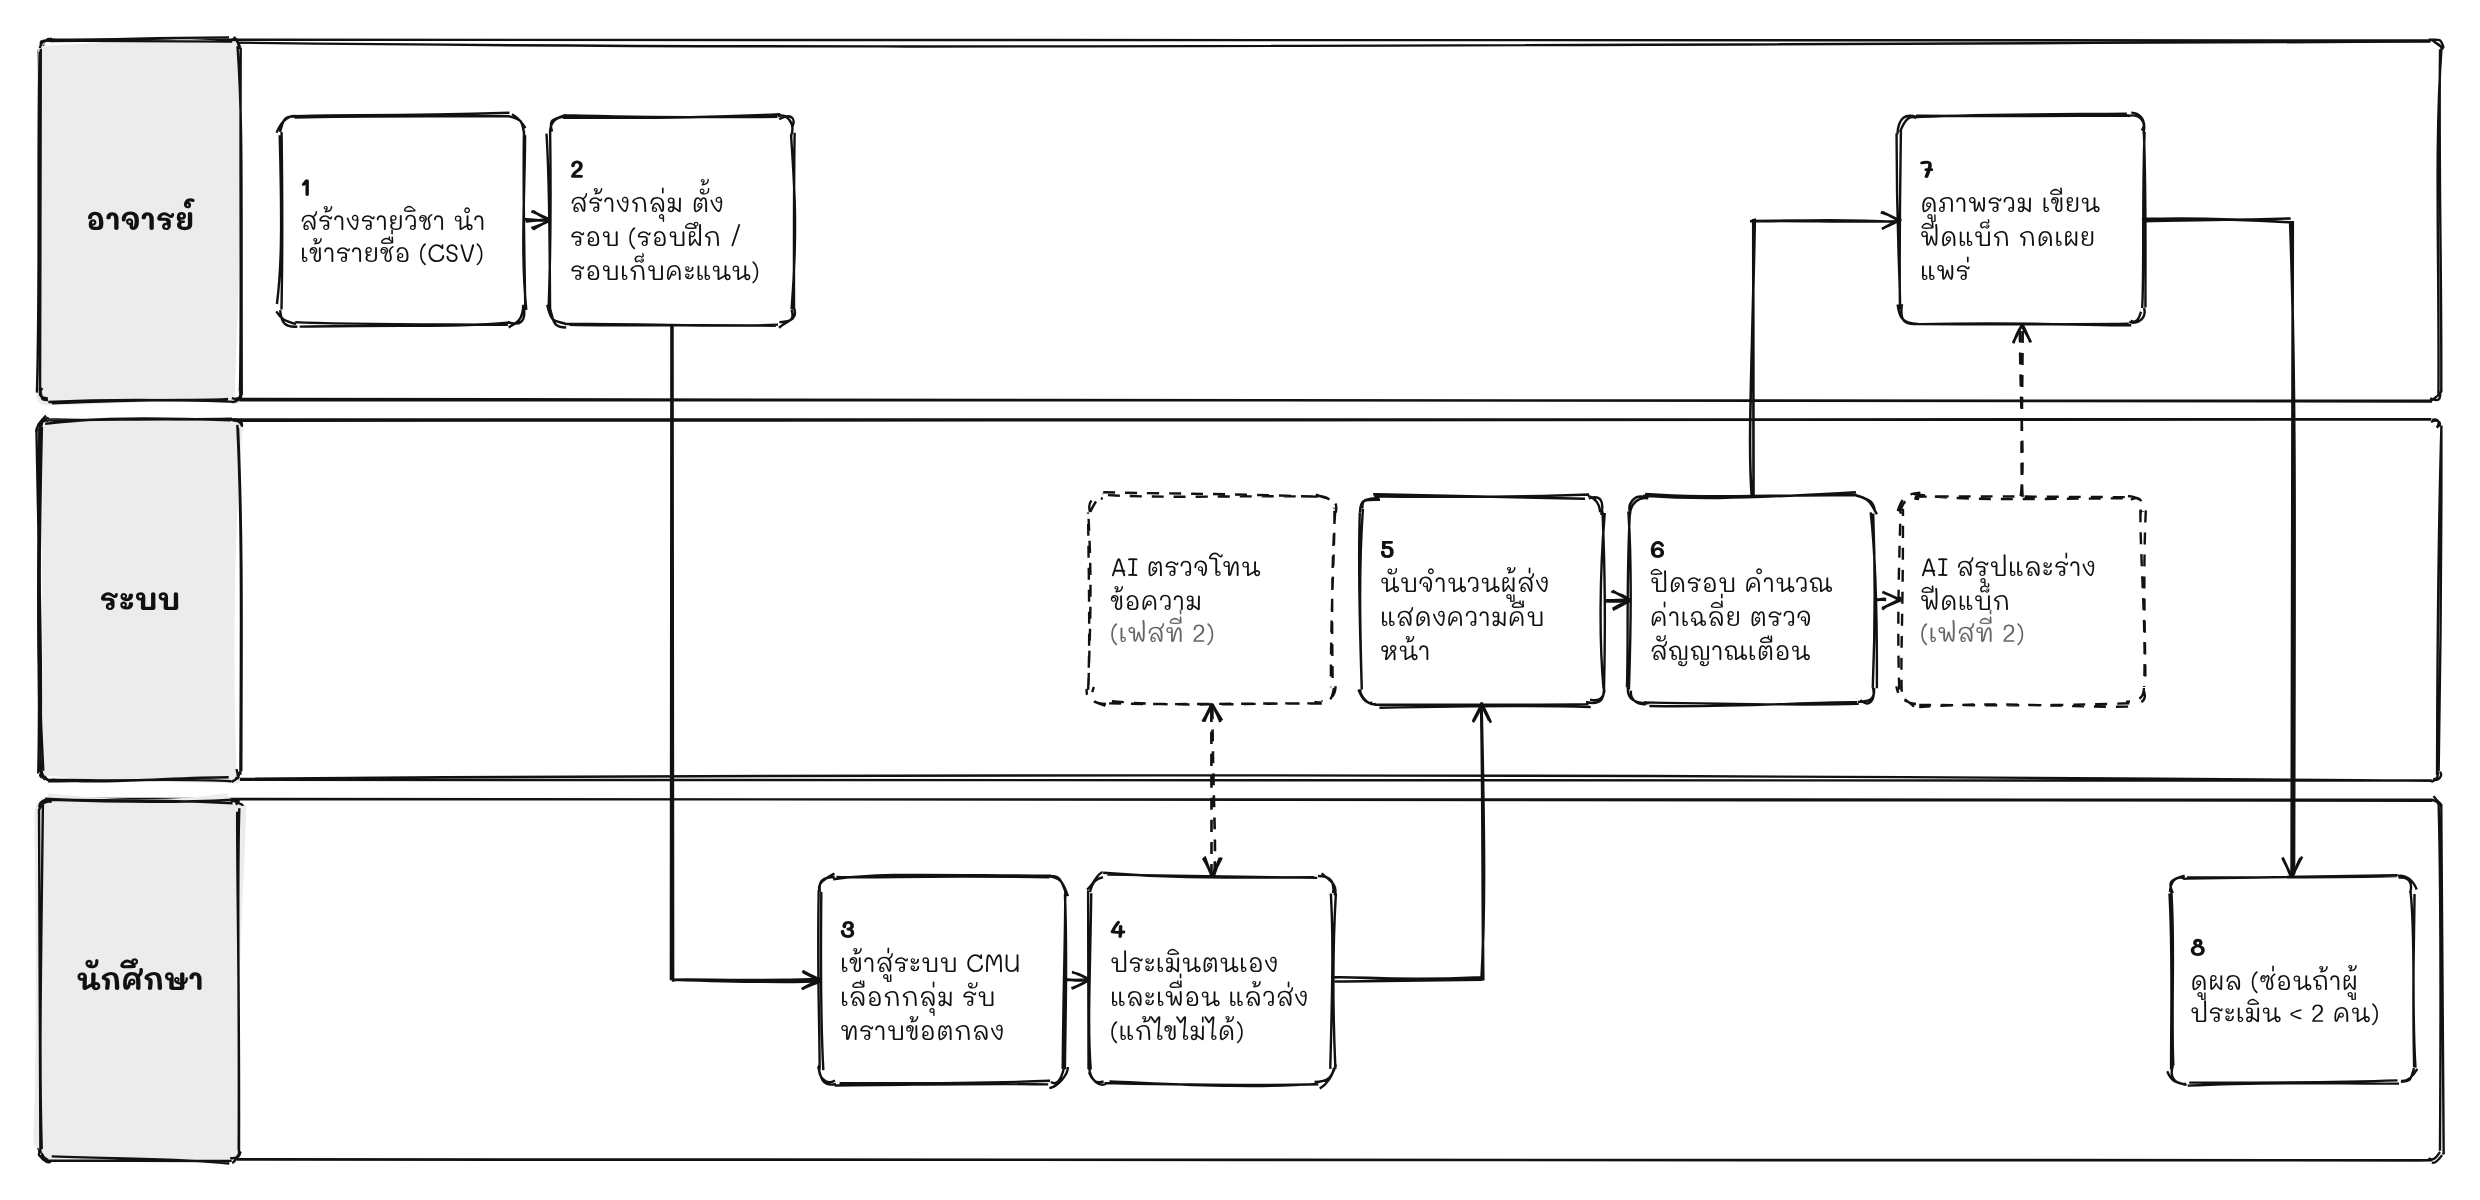
\includegraphics[width=\textwidth]{figures/ch3/fig3-1-swimlane.png}}{\fbox{\parbox{0.8\textwidth}{\centering\vspace{2cm}[วางไฟล์ figures/ch3/fig3-1-swimlane.png]\vspace{2cm}}}}
\caption{ขั้นตอนการทำงานของหนึ่งรอบประเมินแบบ swimlane}\label{fig:ch3-1}
\end{figure}

\subsection{การปกปิดตัวตนและสิทธิ์การมองเห็นข้อมูล}\label{sec:3.5.3}

ระบบไม่เปิดเผยตัวตนของผู้ประเมินต่อเพื่อน เพื่อให้นักศึกษากล้าให้ข้อเสนอแนะอย่างจริงใจ และให้นักศึกษาเห็นเฉพาะข้อมูลของตนเอง เพื่อลดการเปรียบเทียบและแข่งขันกันระหว่างเพื่อน สิทธิ์การมองเห็นข้อมูลแสดงในตารางที่~\ref{tab:ch3-8}

\begin{xltabular}{\textwidth}{|P{0.2\textwidth}|Y|P{0.12\textwidth}|Y|}
\caption{สิทธิ์การมองเห็นข้อมูลของผู้ใช้แต่ละบทบาท}\label{tab:ch3-8}\\
\hline \textbf{ข้อมูล} & \textbf{นักศึกษาเจ้าของข้อมูล} & \textbf{นักศึกษาคนอื่น} & \textbf{อาจารย์} \\ \hline
\endfirsthead
\multicolumn{4}{r}{\small (ต่อ)}\\ \hline \textbf{ข้อมูล} & \textbf{นักศึกษาเจ้าของข้อมูล} & \textbf{นักศึกษาคนอื่น} & \textbf{อาจารย์} \\ \hline
\endhead
คะแนนเฉลี่ยรายด้านที่เพื่อนประเมิน & เห็น เมื่อมีผู้ประเมินอย่างน้อย 2 คนและอาจารย์เผยแพร่แล้ว & ไม่เห็น & เห็น \\ \hline
คะแนนรายคนและชื่อผู้ประเมิน & ไม่เห็น & ไม่เห็น & เห็น เพื่อใช้ติดตามและกลั่นกรอง \\ \hline
ความเห็นปลายเปิด & เห็นหลังอาจารย์เผยแพร่ ในรูปแบบที่อาจารย์เลือก & ไม่เห็น & เห็นทั้งหมด \\ \hline
คะแนนที่ประเมินตนเอง & เห็น & ไม่เห็น & เห็น \\ \hline
สัญญาณเตือนและสถานะการส่ง & ไม่เห็น & ไม่เห็น & เห็น \\ \hline
\end{xltabular}

เงื่อนไขผู้ประเมินขั้นต่ำ 2 คนป้องกันไม่ให้นักศึกษาเดาได้ว่าใครเป็นผู้ประเมินในกรณีที่กลุ่มมีสมาชิกน้อย การบังคับสิทธิ์ทั้งหมดทำที่ฝั่ง API ไม่ใช่เพียงการซ่อนบนหน้าจอ ข้อมูลที่ผู้ใช้ไม่มีสิทธิ์จึงไม่ถูกส่งออกจากเซิร์ฟเวอร์เลย

\subsection{สัญญาณเตือน การเผยแพร่ผล และการสื่อสาร}\label{sec:3.5.4}

ในระยะที่ 1 ระบบสร้างสัญญาณเตือนจากรูปแบบคะแนนตามเงื่อนไขที่กำหนดไว้ (rule-based) เช่น คะแนนเฉลี่ยที่เพื่อนให้ต่ำในด้านใดด้านหนึ่ง คะแนนที่ประเมินตนเองต่างจากที่เพื่อนประเมินมาก หรือยังไม่ส่งแบบประเมิน เพื่อชี้ให้อาจารย์รู้ว่าควรดูแลทีมใดก่อน ฐานข้อมูลเก็บแหล่งที่มาของสัญญาณไว้ด้วย จึงรองรับสัญญาณจากปัญญาประดิษฐ์ (AI) ในระยะที่ 2 ได้โดยไม่ต้องเปลี่ยนโครงสร้าง

ผลการประเมินจะไม่ถึงนักศึกษาโดยอัตโนมัติ อาจารย์เป็นผู้ตรวจทานและกดเผยแพร่ทุกครั้ง โดยเลือกได้ว่าจะแสดงความเห็นของเพื่อนตามจริง หรือแสดงเป็นข้อสรุปที่อาจารย์เขียน การสื่อสารเป็นแบบทางเดียว นักศึกษาตอบกลับความเห็นของเพื่อนในระบบไม่ได้ เพราะการโต้ตอบอาจทำให้สืบทราบตัวตนผู้ประเมินได้ หากนักศึกษามีข้อสงสัยให้สื่อสารผ่านอาจารย์ นอกจากนี้ระบบออกแบบให้ใช้ร่วมกับกิจกรรมในชั้นเรียน เช่น อาจารย์อาจจัดเวลาประมาณ 1 ชั่วโมงให้นักศึกษาพูดคุยเรื่องข้อเสนอแนะกันแบบพบหน้า เพื่อไม่ให้การให้ข้อเสนอแนะผ่านระบบออนไลน์เพียงอย่างเดียวดูห่างเหิน

\section{การออกแบบส่วน AI (ระยะที่ 2)}\label{sec:3.6}

\subsection{ที่มาของการใช้ปัญญาประดิษฐ์}\label{sec:3.6.1}

การเรียนรู้ในปัจจุบันต้องปรับตัวกับการที่ทั้งผู้เรียนและผู้สอนใช้เครื่องมือปัญญาประดิษฐ์ (AI) มากขึ้น ระบบจึงนำปัญญาประดิษฐ์ มาใช้เฉพาะงานที่ปัญญาประดิษฐ์ (AI) ทำได้ดีและลดภาระคนได้จริง คือการอ่านและสรุปข้อความจำนวนมาก และการช่วยเกลาภาษา โดยไม่ให้ปัญญาประดิษฐ์ (AI) ตัดสินใจแทนคน ส่วนปัญญาประดิษฐ์ (AI) จัดอยู่ในการพัฒนาระยะที่ 2 โดยระบบใช้โมเดลภาษา Qwen ผ่าน API และแบ่งเป็น 2 ส่วน ดังรูปที่~\ref{fig:ch3-2}

\begin{figure}[htbp]
\centering
\IfFileExists{figures/ch3/fig3-2-ai.png}{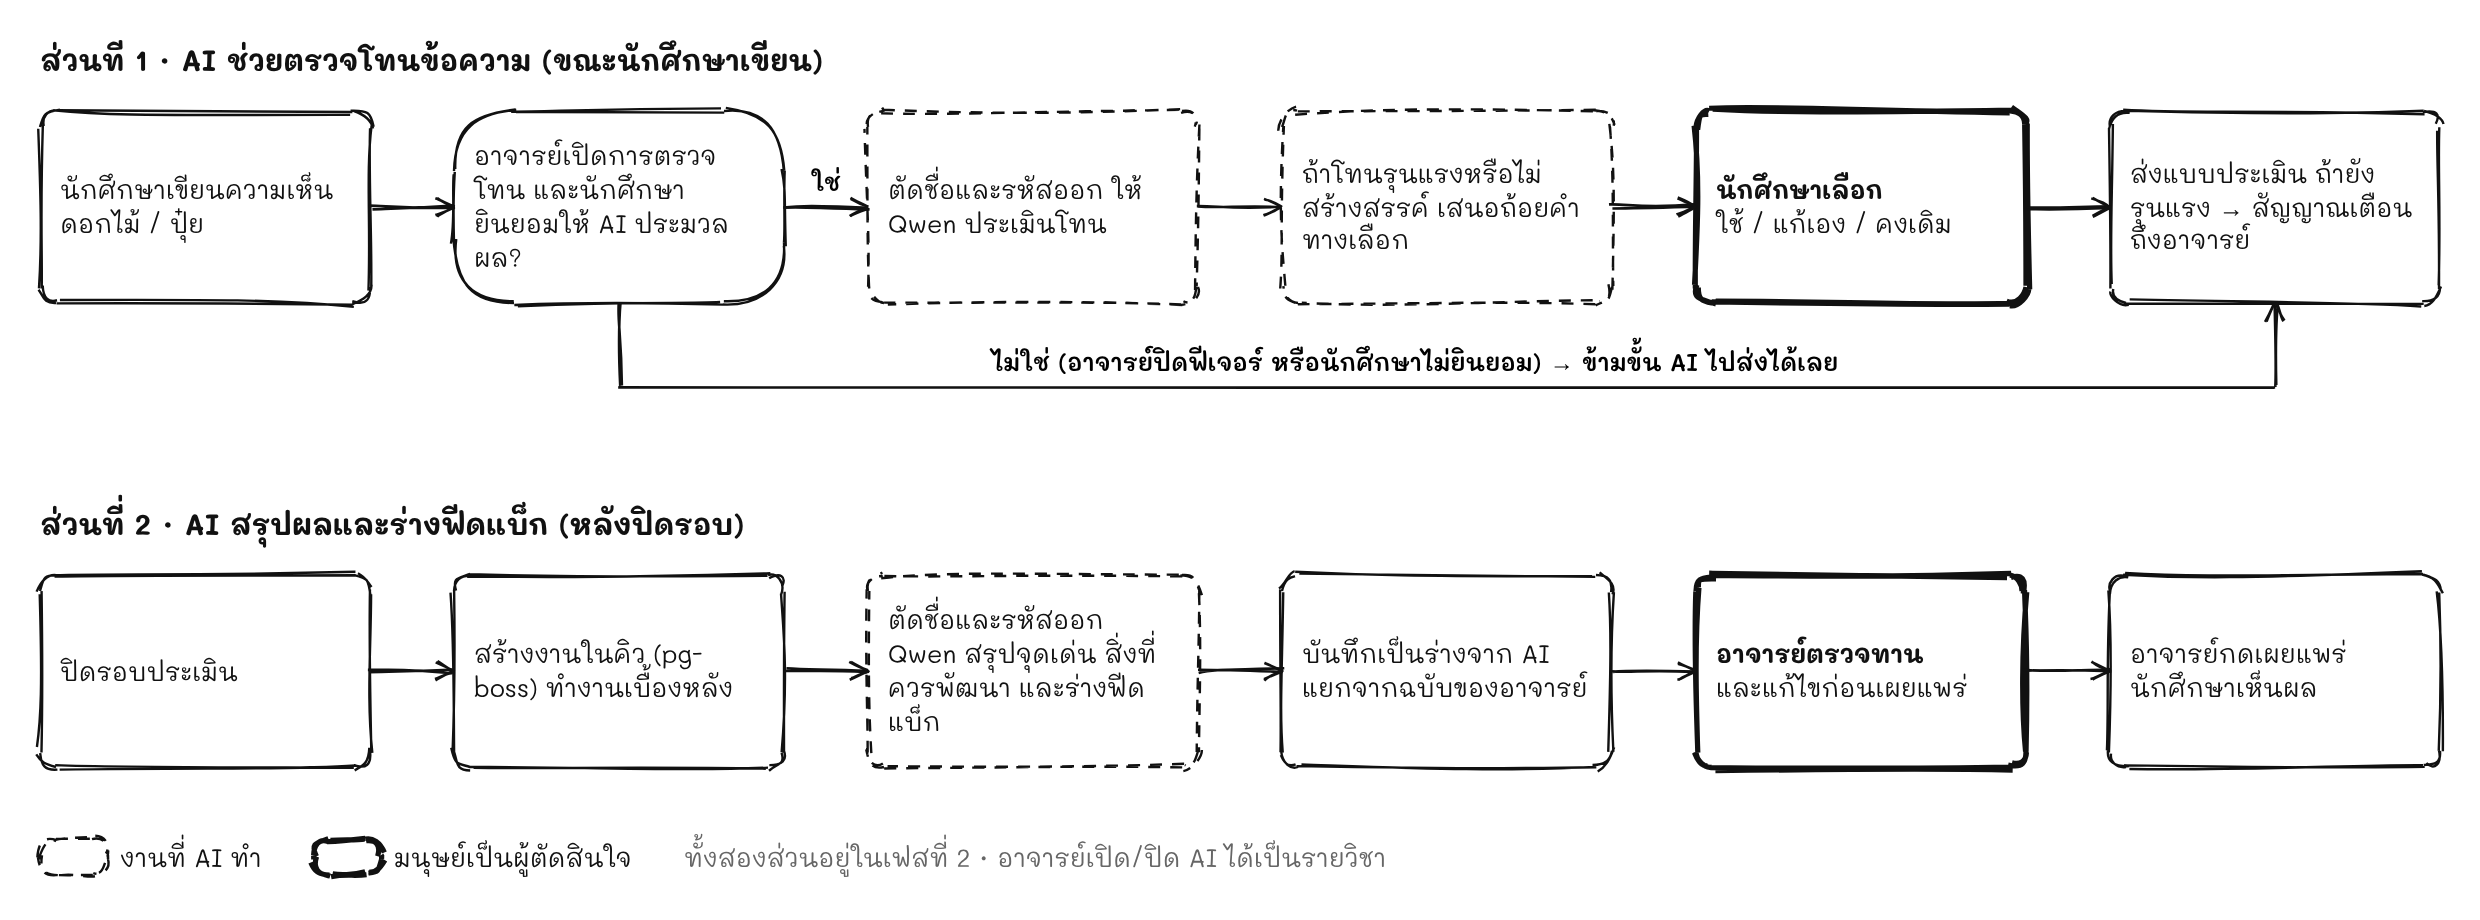
\includegraphics[width=\textwidth]{figures/ch3/fig3-2-ai.png}}{\fbox{\parbox{0.8\textwidth}{\centering\vspace{2cm}[วางไฟล์ figures/ch3/fig3-2-ai.png]\vspace{2cm}}}}
\caption{การทำงานของส่วน AI ทั้ง 2 ส่วน}\label{fig:ch3-2}
\end{figure}

\subsection{ปัญญาประดิษฐ์ช่วยตรวจโทนข้อความ}\label{sec:3.6.2}

อาจารย์เลือกเปิดหรือปิดฟีเจอร์นี้ได้เป็นรายวิชา เมื่อเปิดใช้งาน ขณะนักศึกษาเขียนความเห็นปลายเปิด ระบบส่งข้อความให้โมเดลประเมินโทน หากข้อความมีลักษณะรุนแรง ตำหนิตัวบุคคล หรือไม่สร้างสรรค์ ระบบจะแสดงคำเตือนพร้อมเสนอถ้อยคำทางเลือกที่สื่อประเด็นเดิมอย่างสร้างสรรค์ นักศึกษาเป็นผู้ตัดสินใจเองว่าจะใช้ถ้อยคำที่เสนอ แก้ไขเอง หรือคงข้อความเดิม ระบบไม่เปลี่ยนข้อความให้โดยอัตโนมัติ หากข้อความที่ส่งแล้วยังมีโทนรุนแรง ระบบจะบันทึกเป็นสัญญาณเตือนให้อาจารย์เห็น หากอาจารย์ปิดฟีเจอร์นี้ นักศึกษาจะเขียนและส่งความเห็นได้ตามปกติโดยไม่ผ่านการตรวจโทน

\subsection{ปัญญาประดิษฐ์สรุปผลและร่างข้อเสนอแนะ}\label{sec:3.6.3}

เมื่อปิดรอบประเมิน ระบบรวบรวมความเห็นที่นักศึกษาแต่ละคนได้รับ แล้วส่งให้โมเดลสรุปเป็นจุดเด่นและสิ่งที่ควรพัฒนา พร้อมร่างข้อเสนอแนะถึงนักศึกษาคนนั้น ร่างจากปัญญาประดิษฐ์ (AI) ถูกเก็บแยกจากฉบับที่อาจารย์แก้ไข และอาจารย์ต้องตรวจทานก่อนเผยแพร่ทุกครั้ง การประมวลผลทำผ่านคิวงานเบื้องหลัง ผู้ใช้จึงไม่ต้องรอระหว่างที่โมเดลทำงาน

\subsection{หลักการกำกับการใช้ปัญญาประดิษฐ์ (AI)}\label{sec:3.6.4}

\begin{itemize}
  \item มนุษย์ตัดสินใจขั้นสุดท้ายเสมอ (human-in-the-loop): AI ทำหน้าที่เสนอ ส่วนนักศึกษาและอาจารย์เป็นผู้เลือก
  \item เปิดหรือปิดได้: อาจารย์เปิดหรือปิดฟีเจอร์ปัญญาประดิษฐ์ (AI) ได้เป็นรายวิชา และข้อความของนักศึกษาจะถูกส่งให้ปัญญาประดิษฐ์ (AI) เฉพาะเมื่อนักศึกษายินยอมในส่วนทางเลือก (หัวข้อ~\ref{sec:3.9.2})
  \item ลดข้อมูลที่ส่งออก: ส่งเฉพาะข้อความที่ต้องประมวลผล โดยไม่ส่งชื่อหรือรหัสนักศึกษาไปยังผู้ให้บริการโมเดล
  \item ยอมรับข้อจำกัด: โมเดลอาจตีความภาษาไทยผิด โดยเฉพาะถ้อยคำประชดประชันซึ่งจัดเป็นงานในระยะที่ 3 นี่คือเหตุผลที่ระบบไม่ให้ปัญญาประดิษฐ์ (AI) ตัดสินใจเอง
\end{itemize}

\section{สถาปัตยกรรมระบบและฐานข้อมูล}\label{sec:3.7}

\subsection{ภาพรวมสถาปัตยกรรม}\label{sec:3.7.1}

ระบบเป็นเว็บแอปพลิเคชันที่แยกส่วนหน้า (frontend) และส่วนหลัง (backend) ออกจากกัน และสื่อสารกันผ่าน REST API ด้วยข้อมูลรูปแบบ JSON องค์ประกอบหลักแสดงในรูปที่~\ref{fig:ch3-3} ดังนี้

\begin{itemize}
  \item ส่วนหน้า: React 19, Vite และ TypeScript จัดหน้าตาด้วย Tailwind CSS จัดการข้อมูลจากเซิร์ฟเวอร์ด้วย TanStack Query และจัดการสถานะภายในหน้าเว็บด้วย Zustand
  \item เว็บเซิร์ฟเวอร์: nginx ให้บริการไฟล์ของส่วนหน้า ทำหน้าที่ reverse proxy ไปยัง API และจัดการ HTTPS
  \item ส่วนหลัง: Node.js และ Express 5 เข้าถึงฐานข้อมูลผ่าน Drizzle ORM และกำหนดสัญญาการเชื่อมต่อ API ด้วย OpenAPI
  \item ฐานข้อมูล: PostgreSQL เก็บข้อมูลของระบบ เซสชันผู้ใช้ และคิวงานเบื้องหลัง (pg-boss)
  \item Worker และบริการ AI (เฟสที่ 2): worker ดึงงานจากคิวไปเรียกโมเดล Qwen ผ่าน API แล้วบันทึกผลกลับลงฐานข้อมูล
\end{itemize}

คณะผู้จัดทำเลือกใช้ PostgreSQL เป็นทั้งที่เก็บเซสชันและคิวงาน แทนการเพิ่ม Redis และ BullMQ ซึ่งเป็นอีกทางเลือกหนึ่ง เพื่อลดจำนวนบริการที่ต้องดูแลและใช้ทรัพยากรน้อยลง ทางเลือกนี้เหมาะกับข้อจำกัดของเซิร์ฟเวอร์ขนาด 2 vCPU หน่วยความจำ 4 GB ตามงบประมาณของโครงงาน และปริมาณงานของระบบในระดับรายวิชาซึ่งไม่ได้ต้องการความเร็วที่สูงมาก

\begin{figure}[htbp]
\centering
\IfFileExists{figures/ch3/fig3-3-architecture.png}{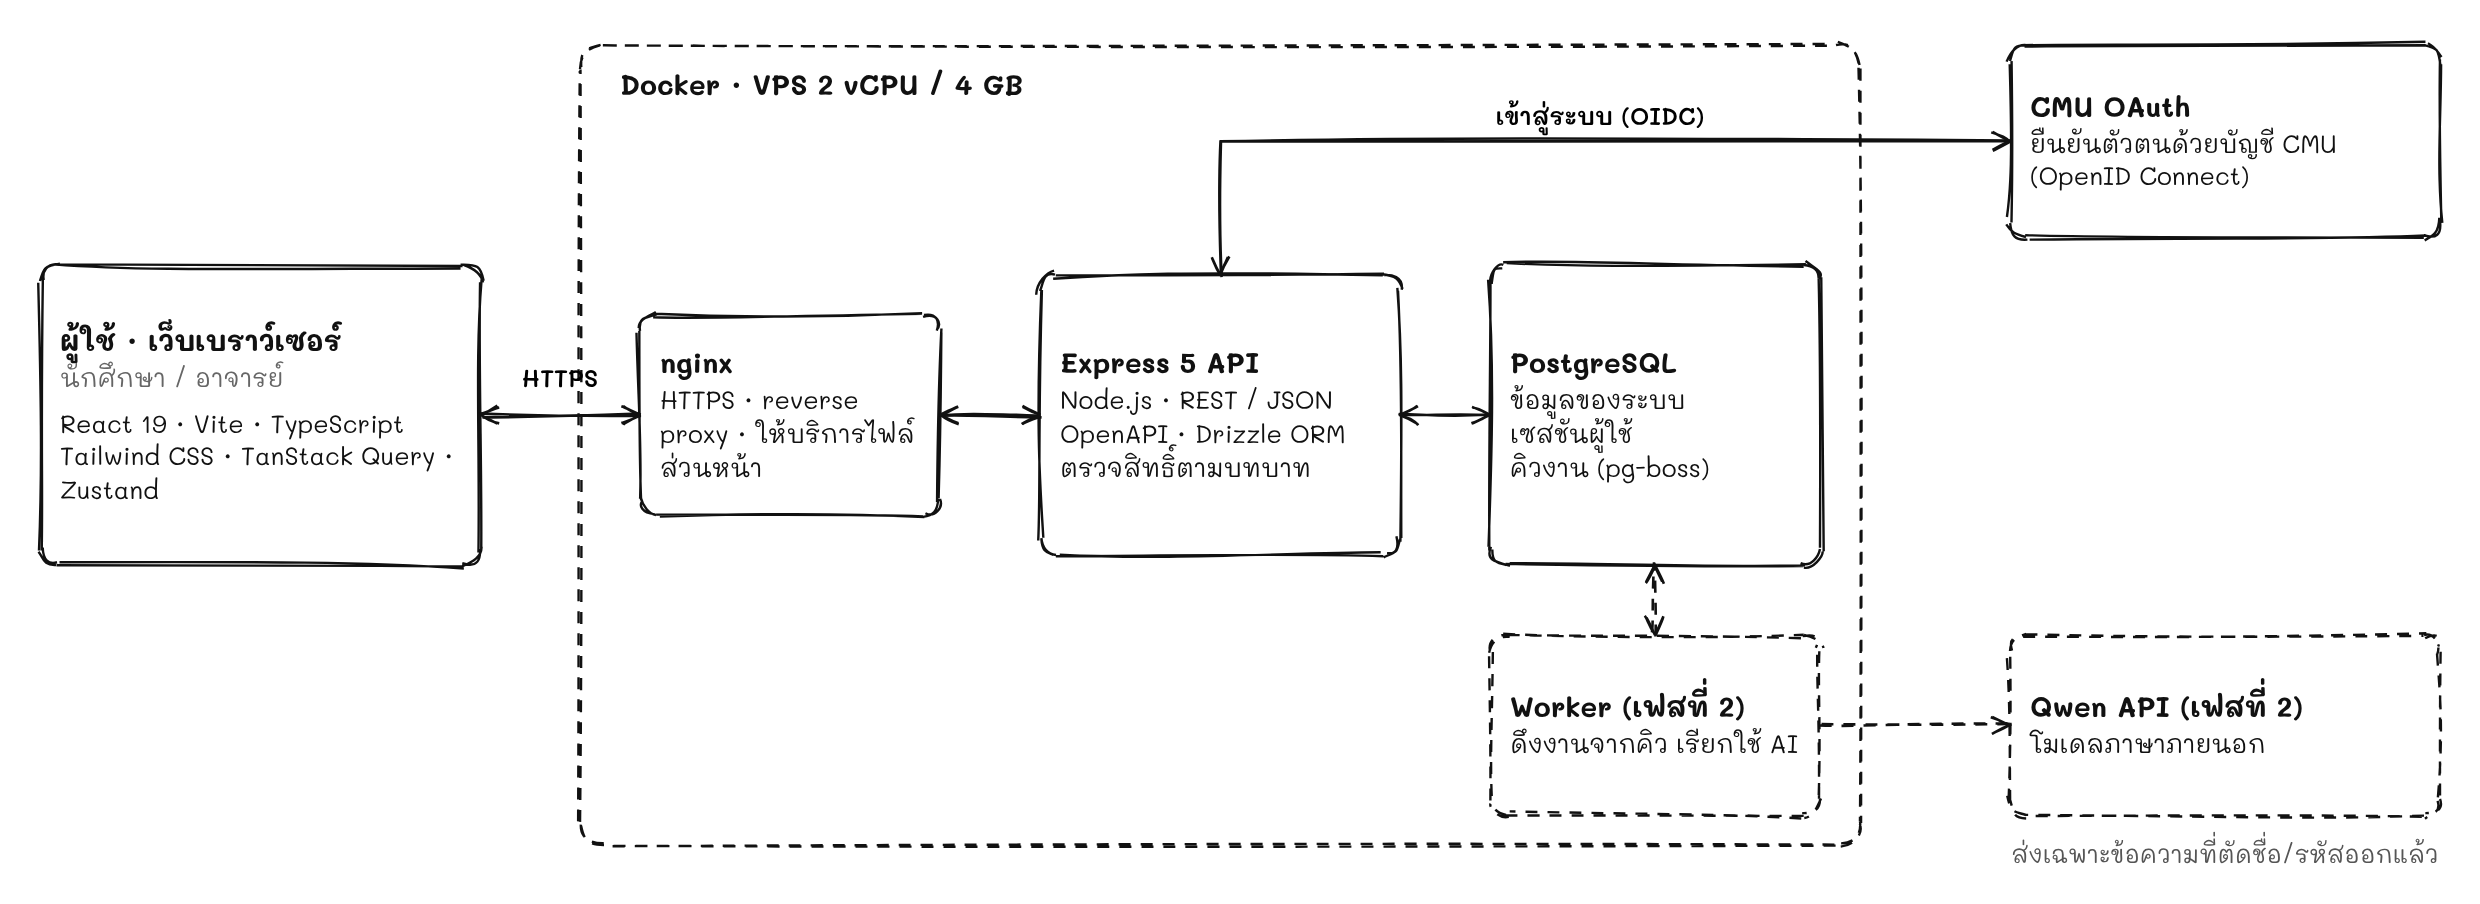
\includegraphics[width=\textwidth]{figures/ch3/fig3-3-architecture.png}}{\fbox{\parbox{0.8\textwidth}{\centering\vspace{2cm}[วางไฟล์ figures/ch3/fig3-3-architecture.png]\vspace{2cm}}}}
\caption{สถาปัตยกรรมของระบบ}\label{fig:ch3-3}
\end{figure}

\subsection{การยืนยันตัวตน}\label{sec:3.7.2}

ผู้ใช้เข้าสู่ระบบด้วยบัญชี CMU ผ่าน CMU OAuth ตามมาตรฐาน OpenID Connect~\cite{sakimura2014oidc} ระบบจึงไม่ต้องเก็บรหัสผ่านของผู้ใช้เอง หลังยืนยันตัวตน เซิร์ฟเวอร์สร้างเซสชันที่เก็บในฐานข้อมูล และส่งคุกกี้เซสชันแบบ HttpOnly และ Secure ให้เบราว์เซอร์ บทบาทของผู้ใช้ในแต่ละรายวิชา (นักศึกษาหรืออาจารย์) ถูกตรวจสอบทุกครั้งที่เรียก API

\subsection{การออกแบบฐานข้อมูล}\label{sec:3.7.3}

ฐานข้อมูลเป็นแบบเชิงสัมพันธ์ ประกอบด้วยตารางที่ระยะที่ 1 ใช้ และตารางที่เตรียมไว้สำหรับระยะถัดไป ได้แก่ ตารางสัญญาณเตือน (flags) และตารางสรุปผล (ai\_feedback\_summaries) สำหรับปัญญาประดิษฐ์ (AI) และตารางบันทึกการซิงก์ข้อมูล (external\_sync\_logs) สำหรับการเชื่อมต่อระบบภายนอก ความสัมพันธ์ของข้อมูลแสดงในรูปที่~\ref{fig:ch3-4} โดยมีการตัดสินใจออกแบบที่สำคัญดังนี้

\begin{itemize}
  \item ตารางคะแนน (ratings) ให้ช่องผู้ถูกประเมินเป็นค่าว่างได้ เพื่อรองรับคำถามระดับทีมที่ไม่ได้ประเมินบุคคลใดบุคคลหนึ่ง
  \item ตารางสรุปผล (ai\_feedback\_summaries) เก็บทั้งร่างจากปัญญาประดิษฐ์ (AI) และฉบับสุดท้ายที่อาจารย์แก้ไข เพื่อแยกให้เห็นว่าส่วนใดมาจากปัญญาประดิษฐ์ (AI) และส่วนใดผ่านการตรวจทานแล้ว
  \item ตารางความยินยอม (consents) เก็บเวอร์ชันของนโยบายที่ผู้ใช้ยินยอม เพื่อขอความยินยอมใหม่ได้เมื่อนโยบายเปลี่ยน
  \item ตารางสัญญาณเตือน (flags) มีช่องระบุแหล่งที่มาของสัญญาณ เพื่อรองรับทั้งสัญญาณจากเงื่อนไขคะแนนและจากปัญญาประดิษฐ์ (AI)
  \item ตารางรายวิชาและผู้ใช้มีช่องเก็บรหัสอ้างอิงจากระบบภายนอก เพื่อเตรียมเชื่อมต่อ Mango Canvas ในระยะที่ 3 โดยมีตารางบันทึกการซิงก์ข้อมูล (external\_sync\_logs) เก็บผลการนำเข้ารายชื่อและส่งออกคะแนนของแต่ละรายวิชา
  \item ตารางระดับเกณฑ์การให้คะแนน (rubric\_levels) เก็บคำอธิบายพฤติกรรมของแต่ละคะแนนในคำถามแบบให้คะแนน เพื่อให้ผู้ประเมินใช้เกณฑ์เดียวกัน
\end{itemize}

\begin{sidewaysfigure}
\centering
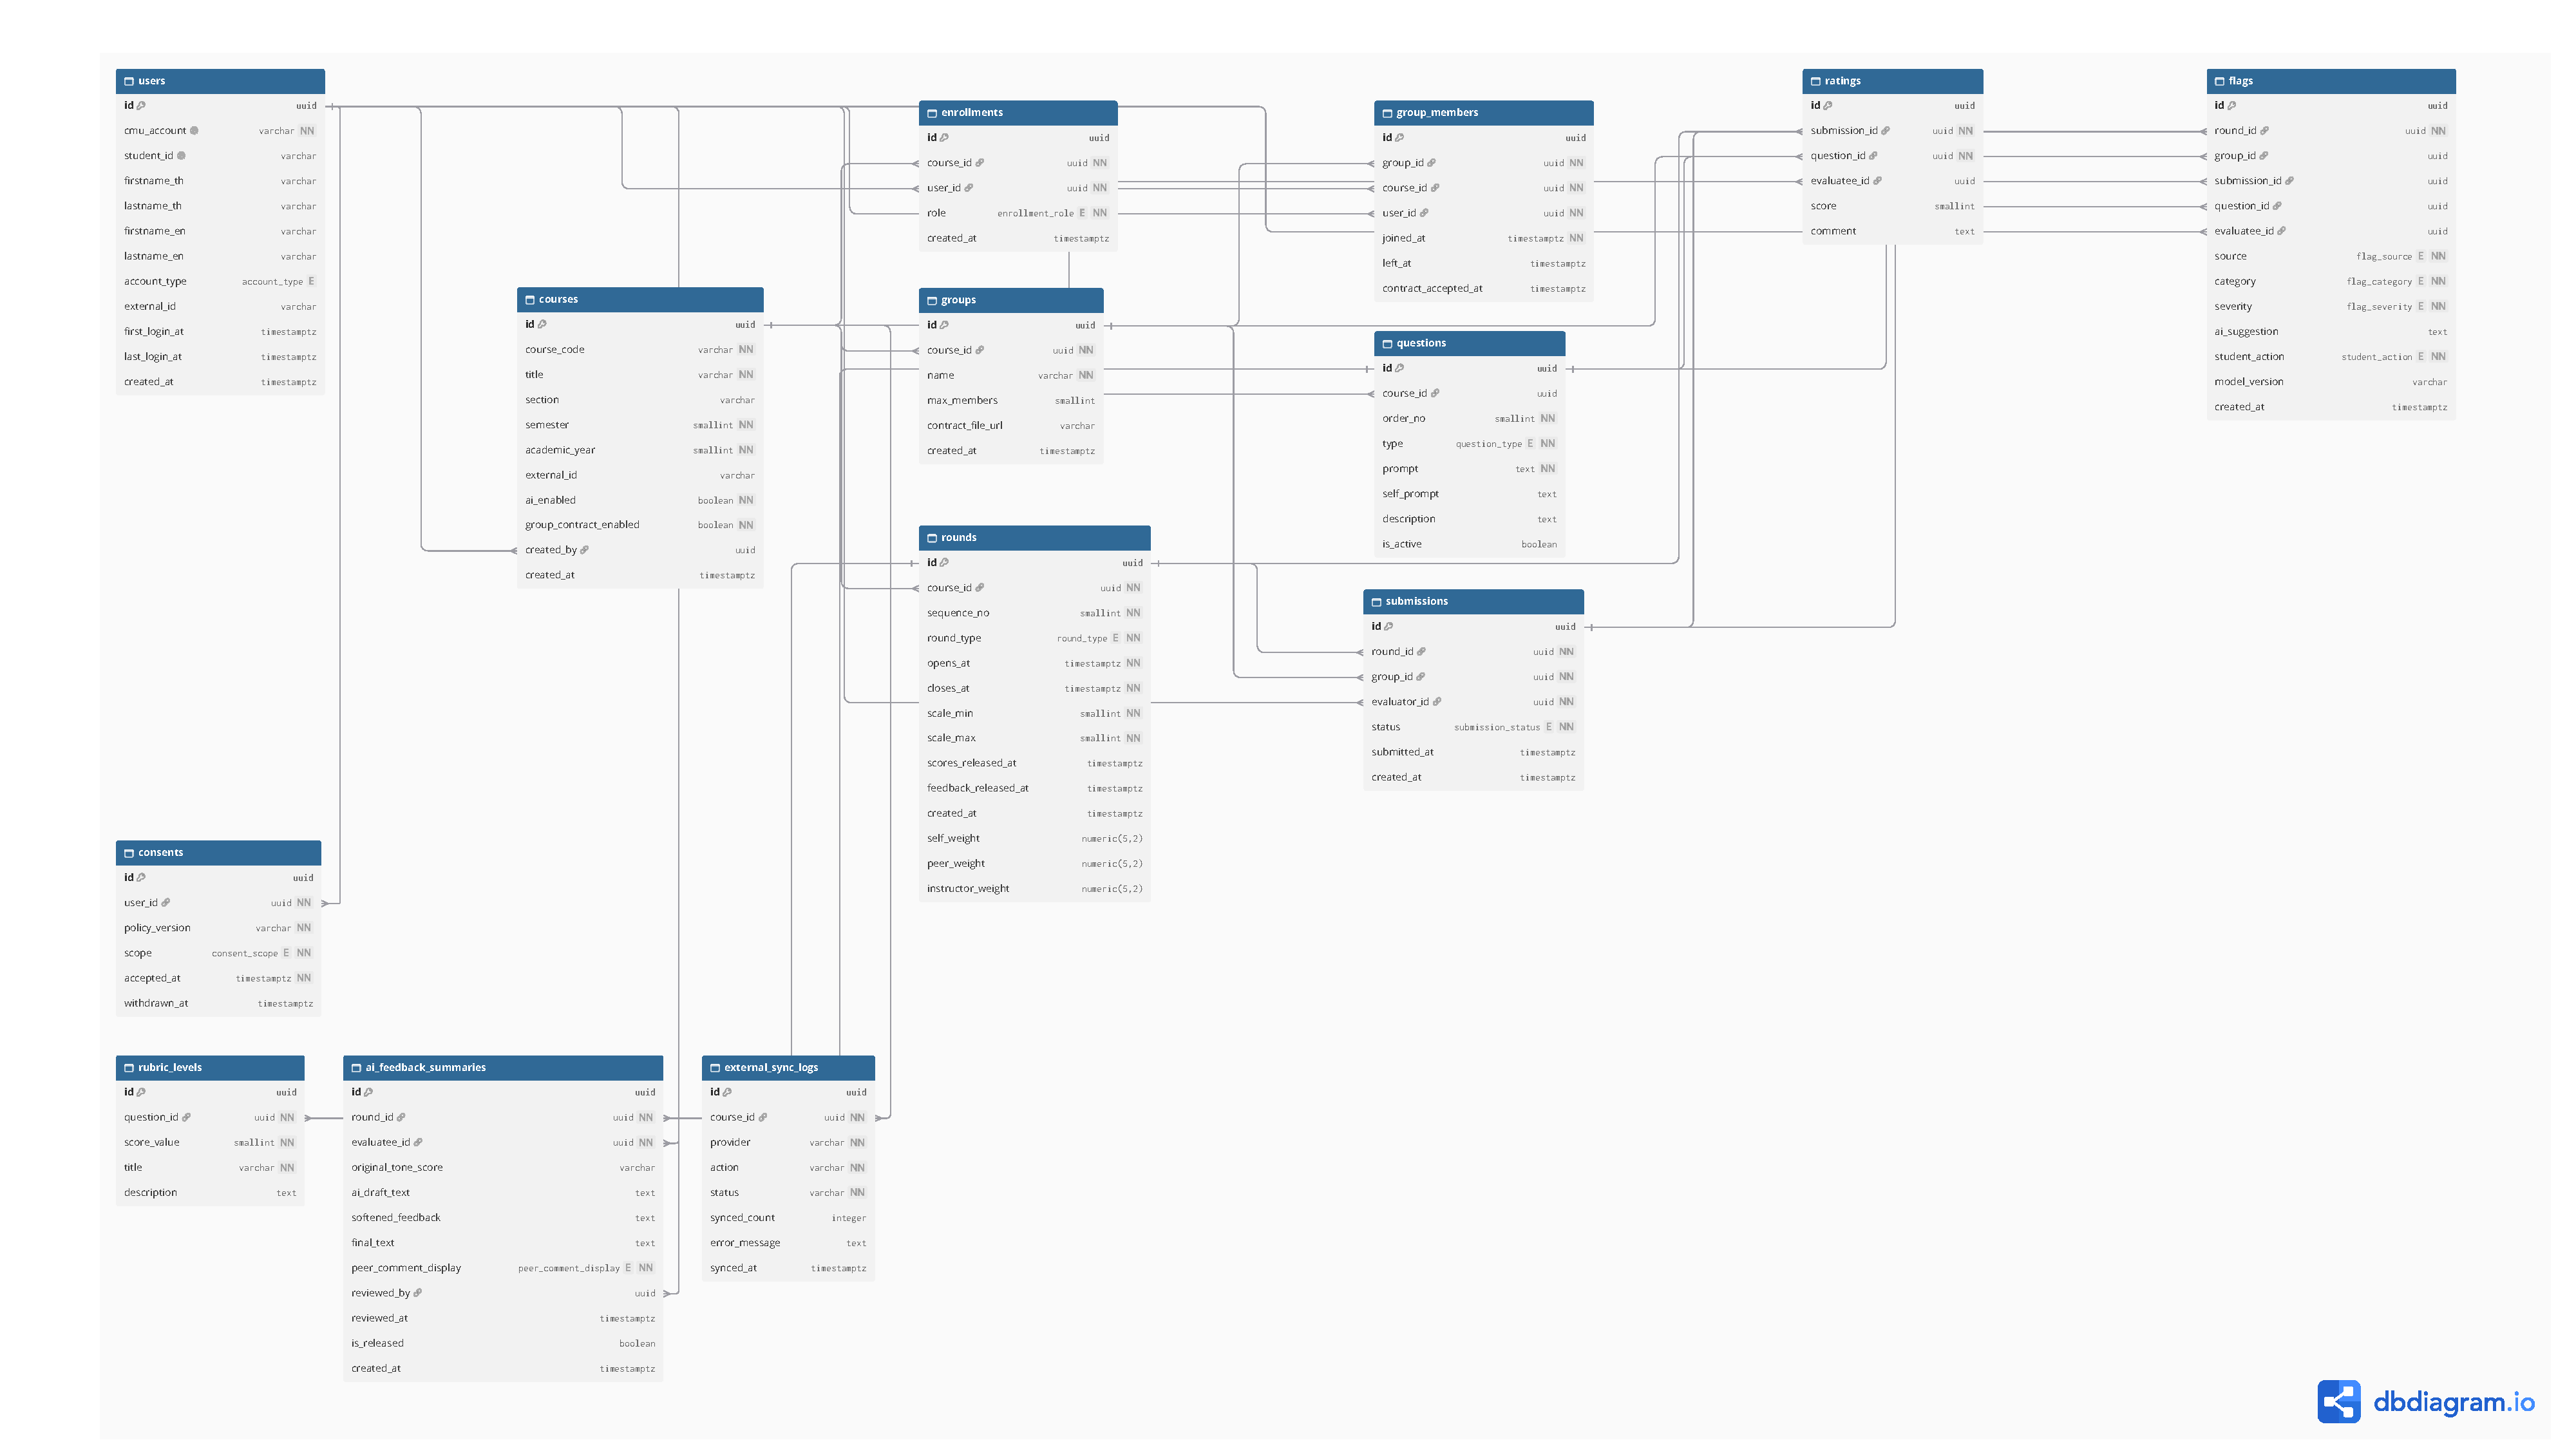
\includegraphics[width=\linewidth]{figures/ch3/fig3-4-er.pdf}
\caption{แผนภาพความสัมพันธ์ของข้อมูล (ER diagram)}\label{fig:ch3-4}
\end{sidewaysfigure}

\subsection{การติดตั้งและการทดสอบ}\label{sec:3.7.4}

ทุกบริการถูกบรรจุเป็น Docker container และติดตั้งบนเซิร์ฟเวอร์เสมือน (VPS) ขนาด 2 vCPU หน่วยความจำ 4 GB การทดสอบใช้ Vitest สำหรับ unit test และ integration test และใช้ Cypress สำหรับ end-to-end test ส่วนการสำรองข้อมูล การตรวจสอบสถานะระบบ และการส่งอีเมล ใช้บริการแบบไม่มีค่าใช้จ่าย

\section{การออกแบบส่วนต่อประสานผู้ใช้}\label{sec:3.8}

\subsection{หลักการออกแบบ}\label{sec:3.8.1}

\begin{itemize}
  \item นำทางตามงาน: แถบเมนูด้านข้างจัดตามงานที่ผู้ใช้ต้องทำ พร้อมตัวเลขแจ้งจำนวนงานค้าง
  \item แสดงสถานะด้วยป้ายสถานะ (status pill) เช่น เปิดรับ ปิดแล้ว และรอเผยแพร่
  \item แบบประเมินแสดงทีละคำถามต่อหน้าจอ เพื่อลดภาระการอ่านและใช้งานบนมือถือได้สะดวก
  \item ออกแบบตามแนวทาง WCAG 2.2~\cite{w3c2023wcag} เช่น ความต่างของสีตัวอักษรกับพื้นหลังที่เพียงพอ การใช้งานด้วยแป้นพิมพ์ และการติดป้ายกำกับช่องกรอกทุกช่อง
\end{itemize}

หน้าจอทั้งหมดออกแบบเป็นต้นแบบความละเอียดต่ำ (low-fidelity wireframe) แบบขาวดำก่อนพัฒนาจริง และใช้ต้นแบบนี้สื่อสารทั้งภายในทีมและกับอาจารย์ผู้ใช้ เพื่อรับความคิดเห็นก่อนลงมือพัฒนา

\subsection{หน้าจอฝั่งนักศึกษา}\label{sec:3.8.2}

ผู้ใช้เข้าสู่ระบบด้วยบัญชี CMU ผ่าน CMU OAuth โดยไม่ต้องสร้างรหัสผ่านใหม่ ดังรูปที่~\ref{fig:ch3-5}

\begin{figure}[htbp]
\centering
\IfFileExists{figures/ch3/fig3-5-login.png}{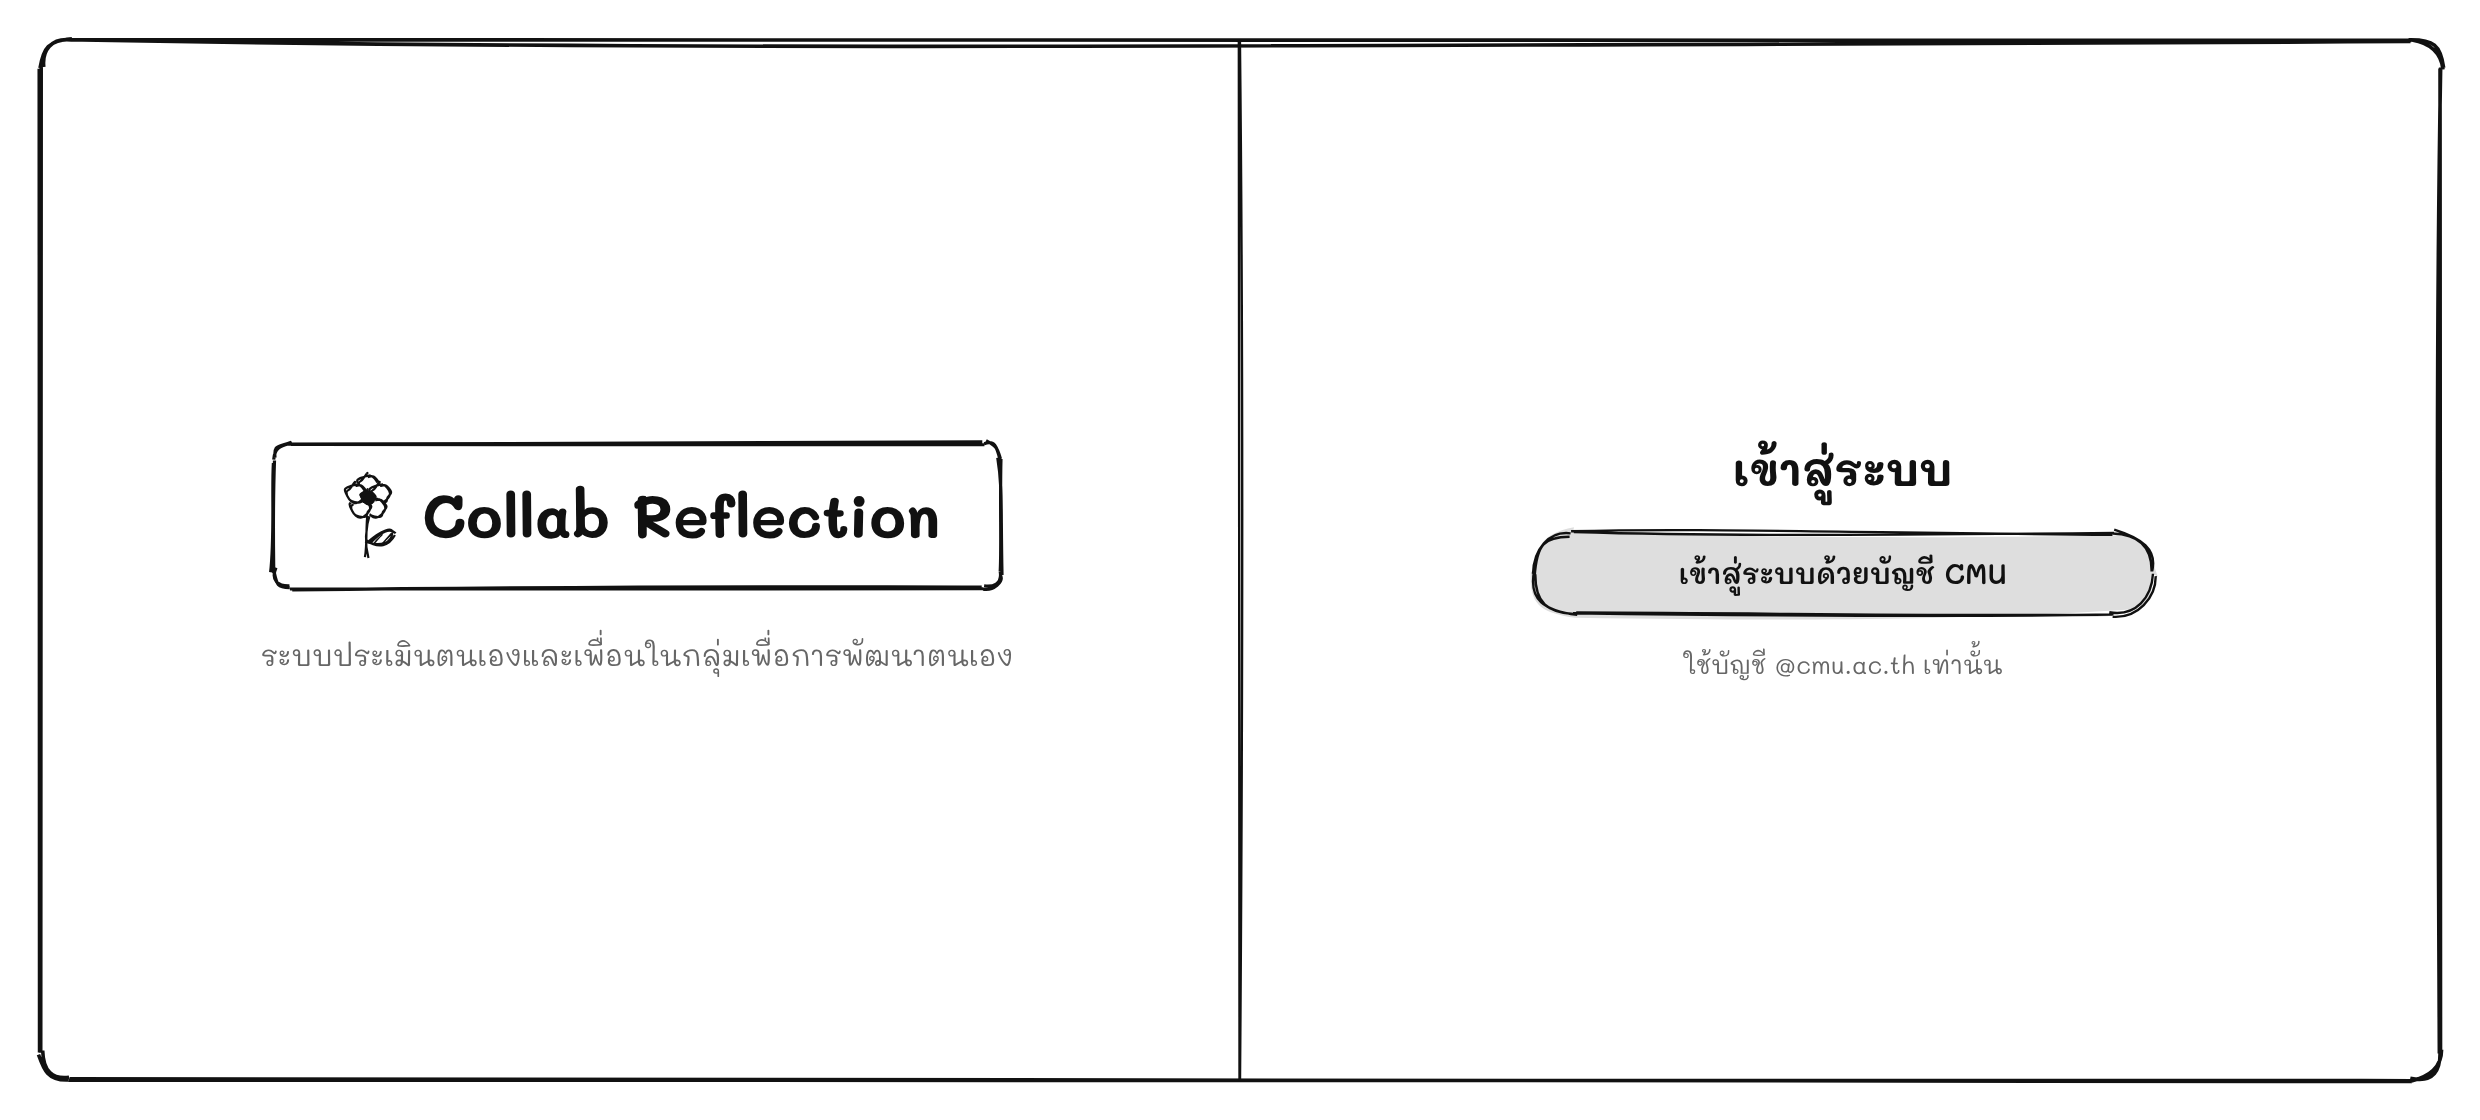
\includegraphics[width=\textwidth]{figures/ch3/fig3-5-login.png}}{\fbox{\parbox{0.8\textwidth}{\centering\vspace{2cm}[วางไฟล์ figures/ch3/fig3-5-login.png]\vspace{2cm}}}}
\caption{หน้าเข้าสู่ระบบ}\label{fig:ch3-5}
\end{figure}

ครั้งแรกที่เข้าใช้งาน นักศึกษาต้องอ่านข้อตกลงการใช้ข้อมูลส่วนบุคคล ซึ่งแบ่งจอเป็น 2 ส่วน ด้านซ้ายย้ำว่าความเห็นถึงเพื่อนจะไม่ระบุชื่อ ด้านขวาแสดงว่าเก็บข้อมูลอะไร ใครเห็น เก็บนานเท่าใด และสิทธิ์ของเจ้าของข้อมูล พร้อมตัวเลือกส่วนจำเป็นและส่วนทางเลือก ดังรูปที่~\ref{fig:ch3-6}

\begin{figure}[htbp]
\centering
\IfFileExists{figures/ch3/fig3-6-consent.png}{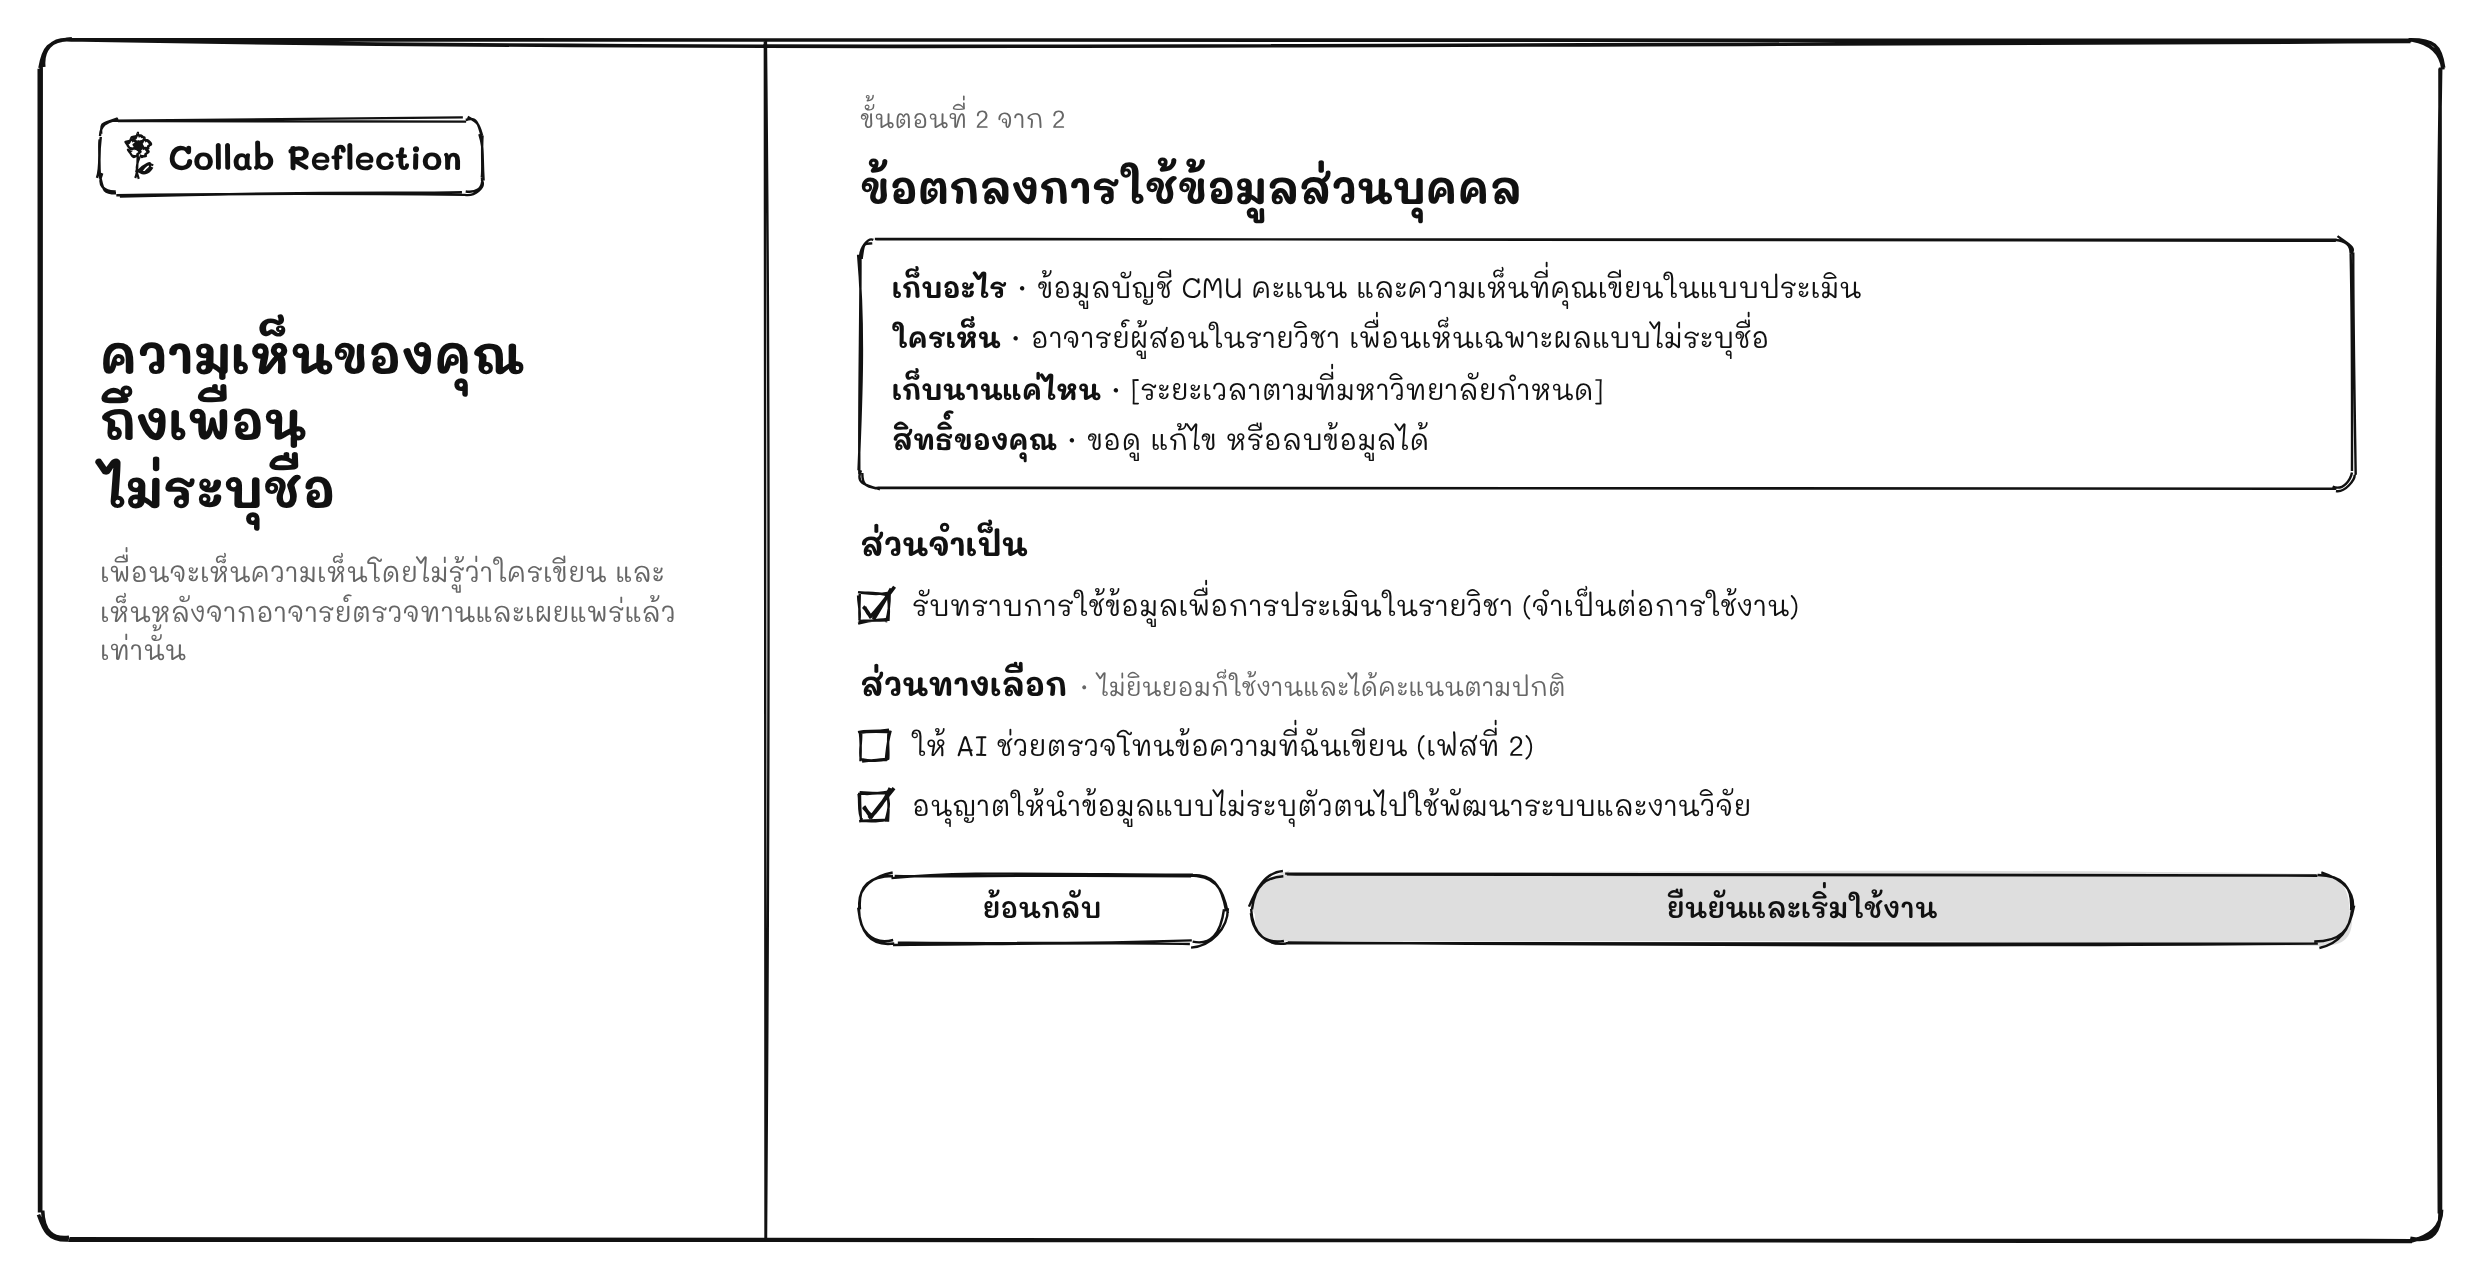
\includegraphics[width=\textwidth]{figures/ch3/fig3-6-consent.png}}{\fbox{\parbox{0.8\textwidth}{\centering\vspace{2cm}[วางไฟล์ figures/ch3/fig3-6-consent.png]\vspace{2cm}}}}
\caption{หน้าข้อตกลงการใช้ข้อมูลส่วนบุคคล}\label{fig:ch3-6}
\end{figure}

หน้ารายวิชาแสดงกลุ่มของนักศึกษา ข้อตกลงกลุ่ม และรายการรอบประเมิน โดยทุกรอบมีป้ายบอกว่าเป็นรอบฝึกหรือรอบเก็บคะแนน พร้อมสถานะของรอบ ดังรูปที่~\ref{fig:ch3-7}

\begin{figure}[htbp]
\centering
\IfFileExists{figures/ch3/fig3-7-student-course.png}{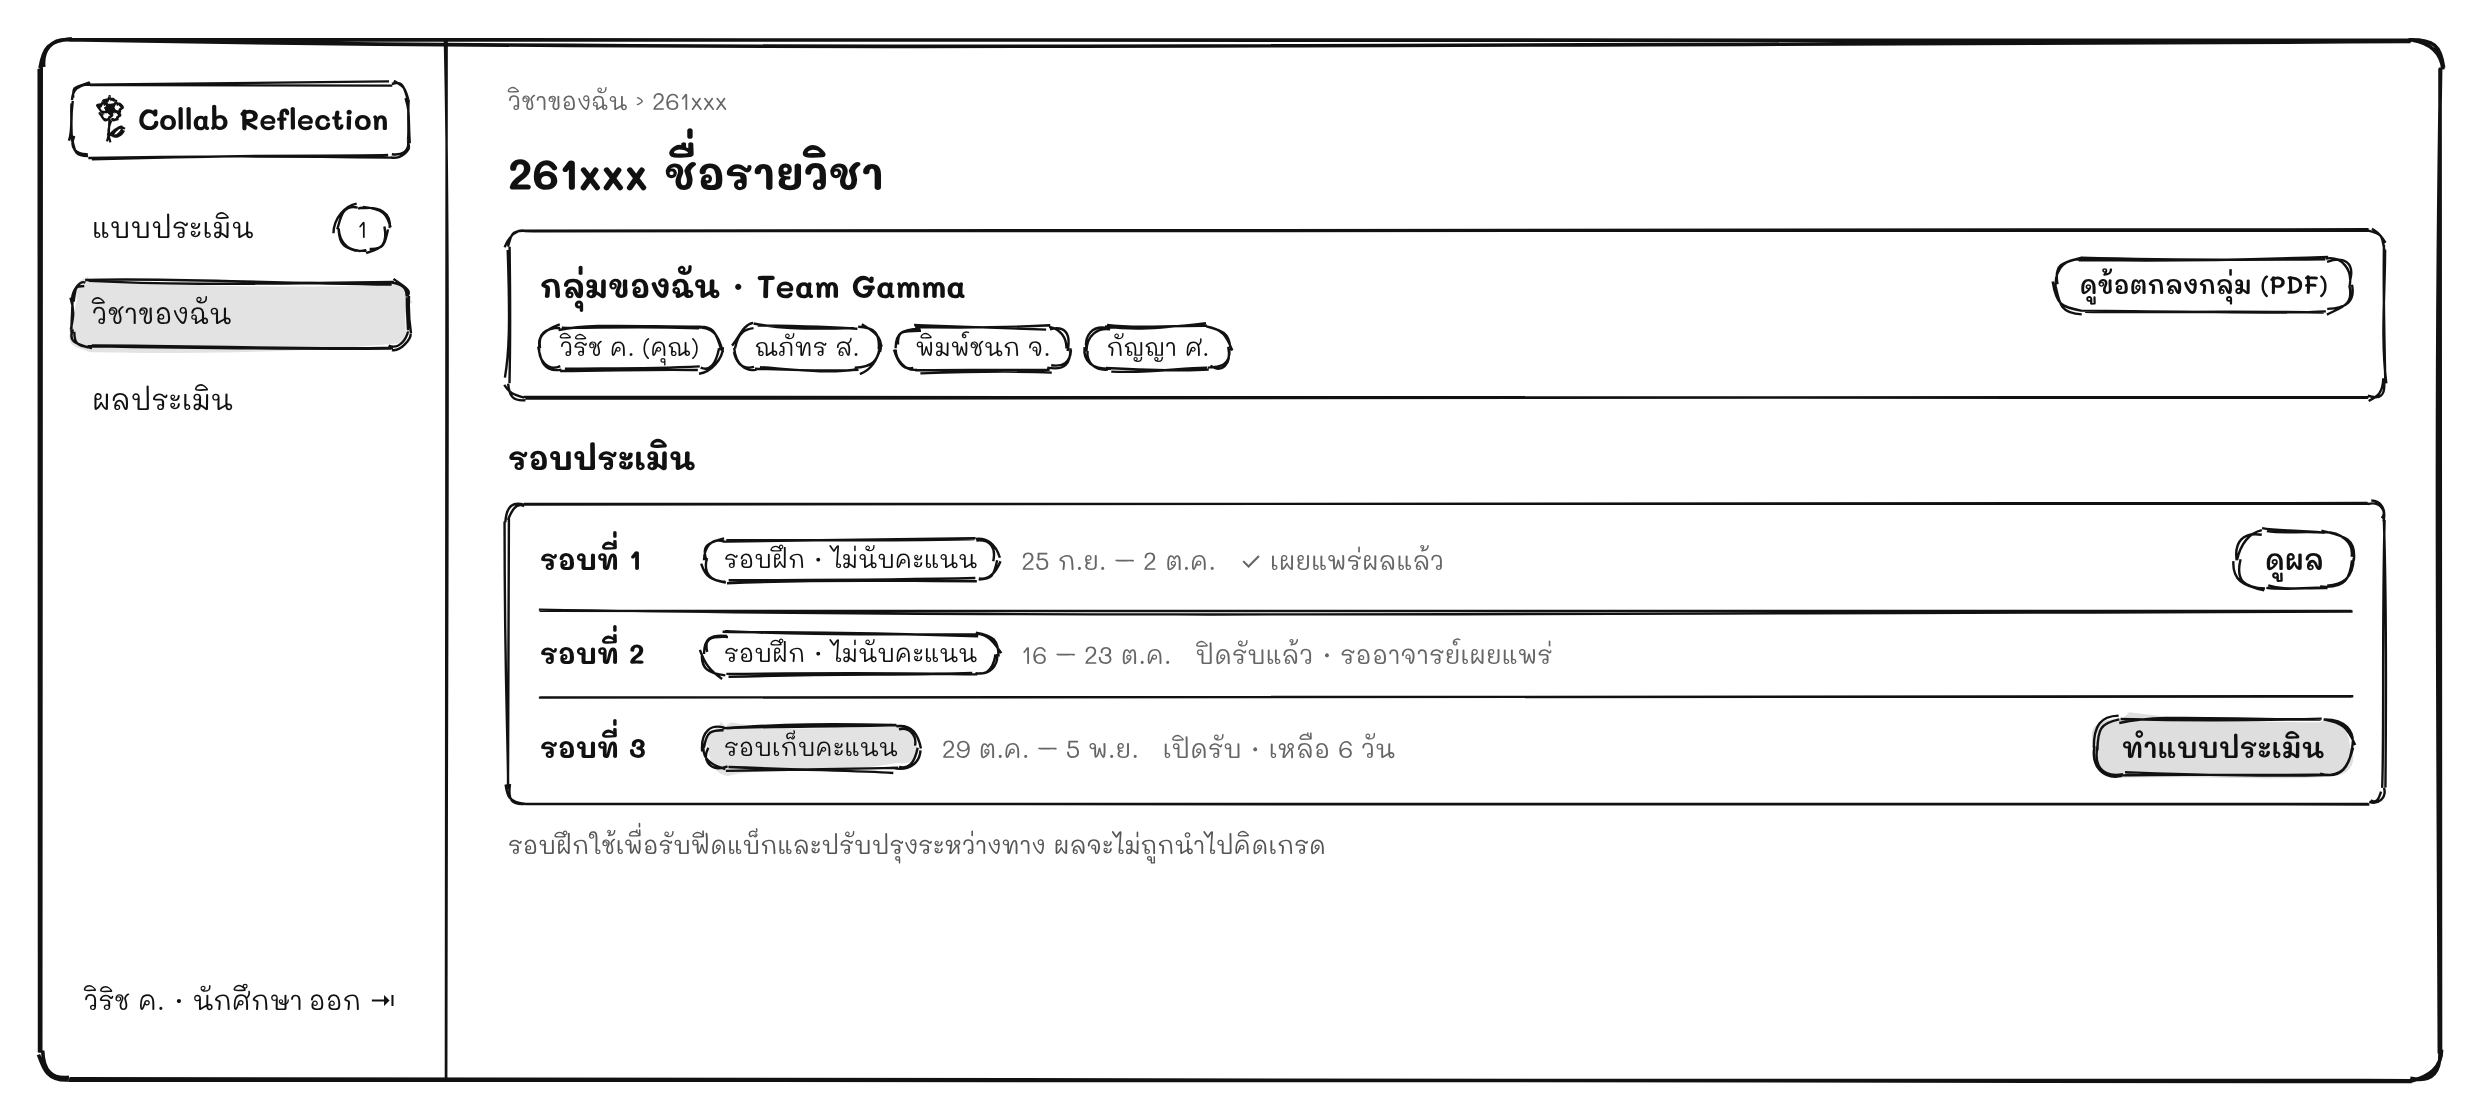
\includegraphics[width=\textwidth]{figures/ch3/fig3-7-student-course.png}}{\fbox{\parbox{0.8\textwidth}{\centering\vspace{2cm}[วางไฟล์ figures/ch3/fig3-7-student-course.png]\vspace{2cm}}}}
\caption{หน้ารายวิชาและรอบประเมินของนักศึกษา}\label{fig:ch3-7}
\end{figure}

แบบประเมินแสดงทีละด้านต่อหน้าจอ ด้านบนมีคำอธิบายพฤติกรรมของระดับ 1, 3 และ 5 ให้นักศึกษาให้คะแนนสมาชิกทุกคนรวมถึงตนเอง และด้านขวามีแถบแสดงขั้นตอนทั้ง 7 ขั้น ดังรูปที่~\ref{fig:ch3-8}

\begin{figure}[htbp]
\centering
\IfFileExists{figures/ch3/fig3-8-student-rating.png}{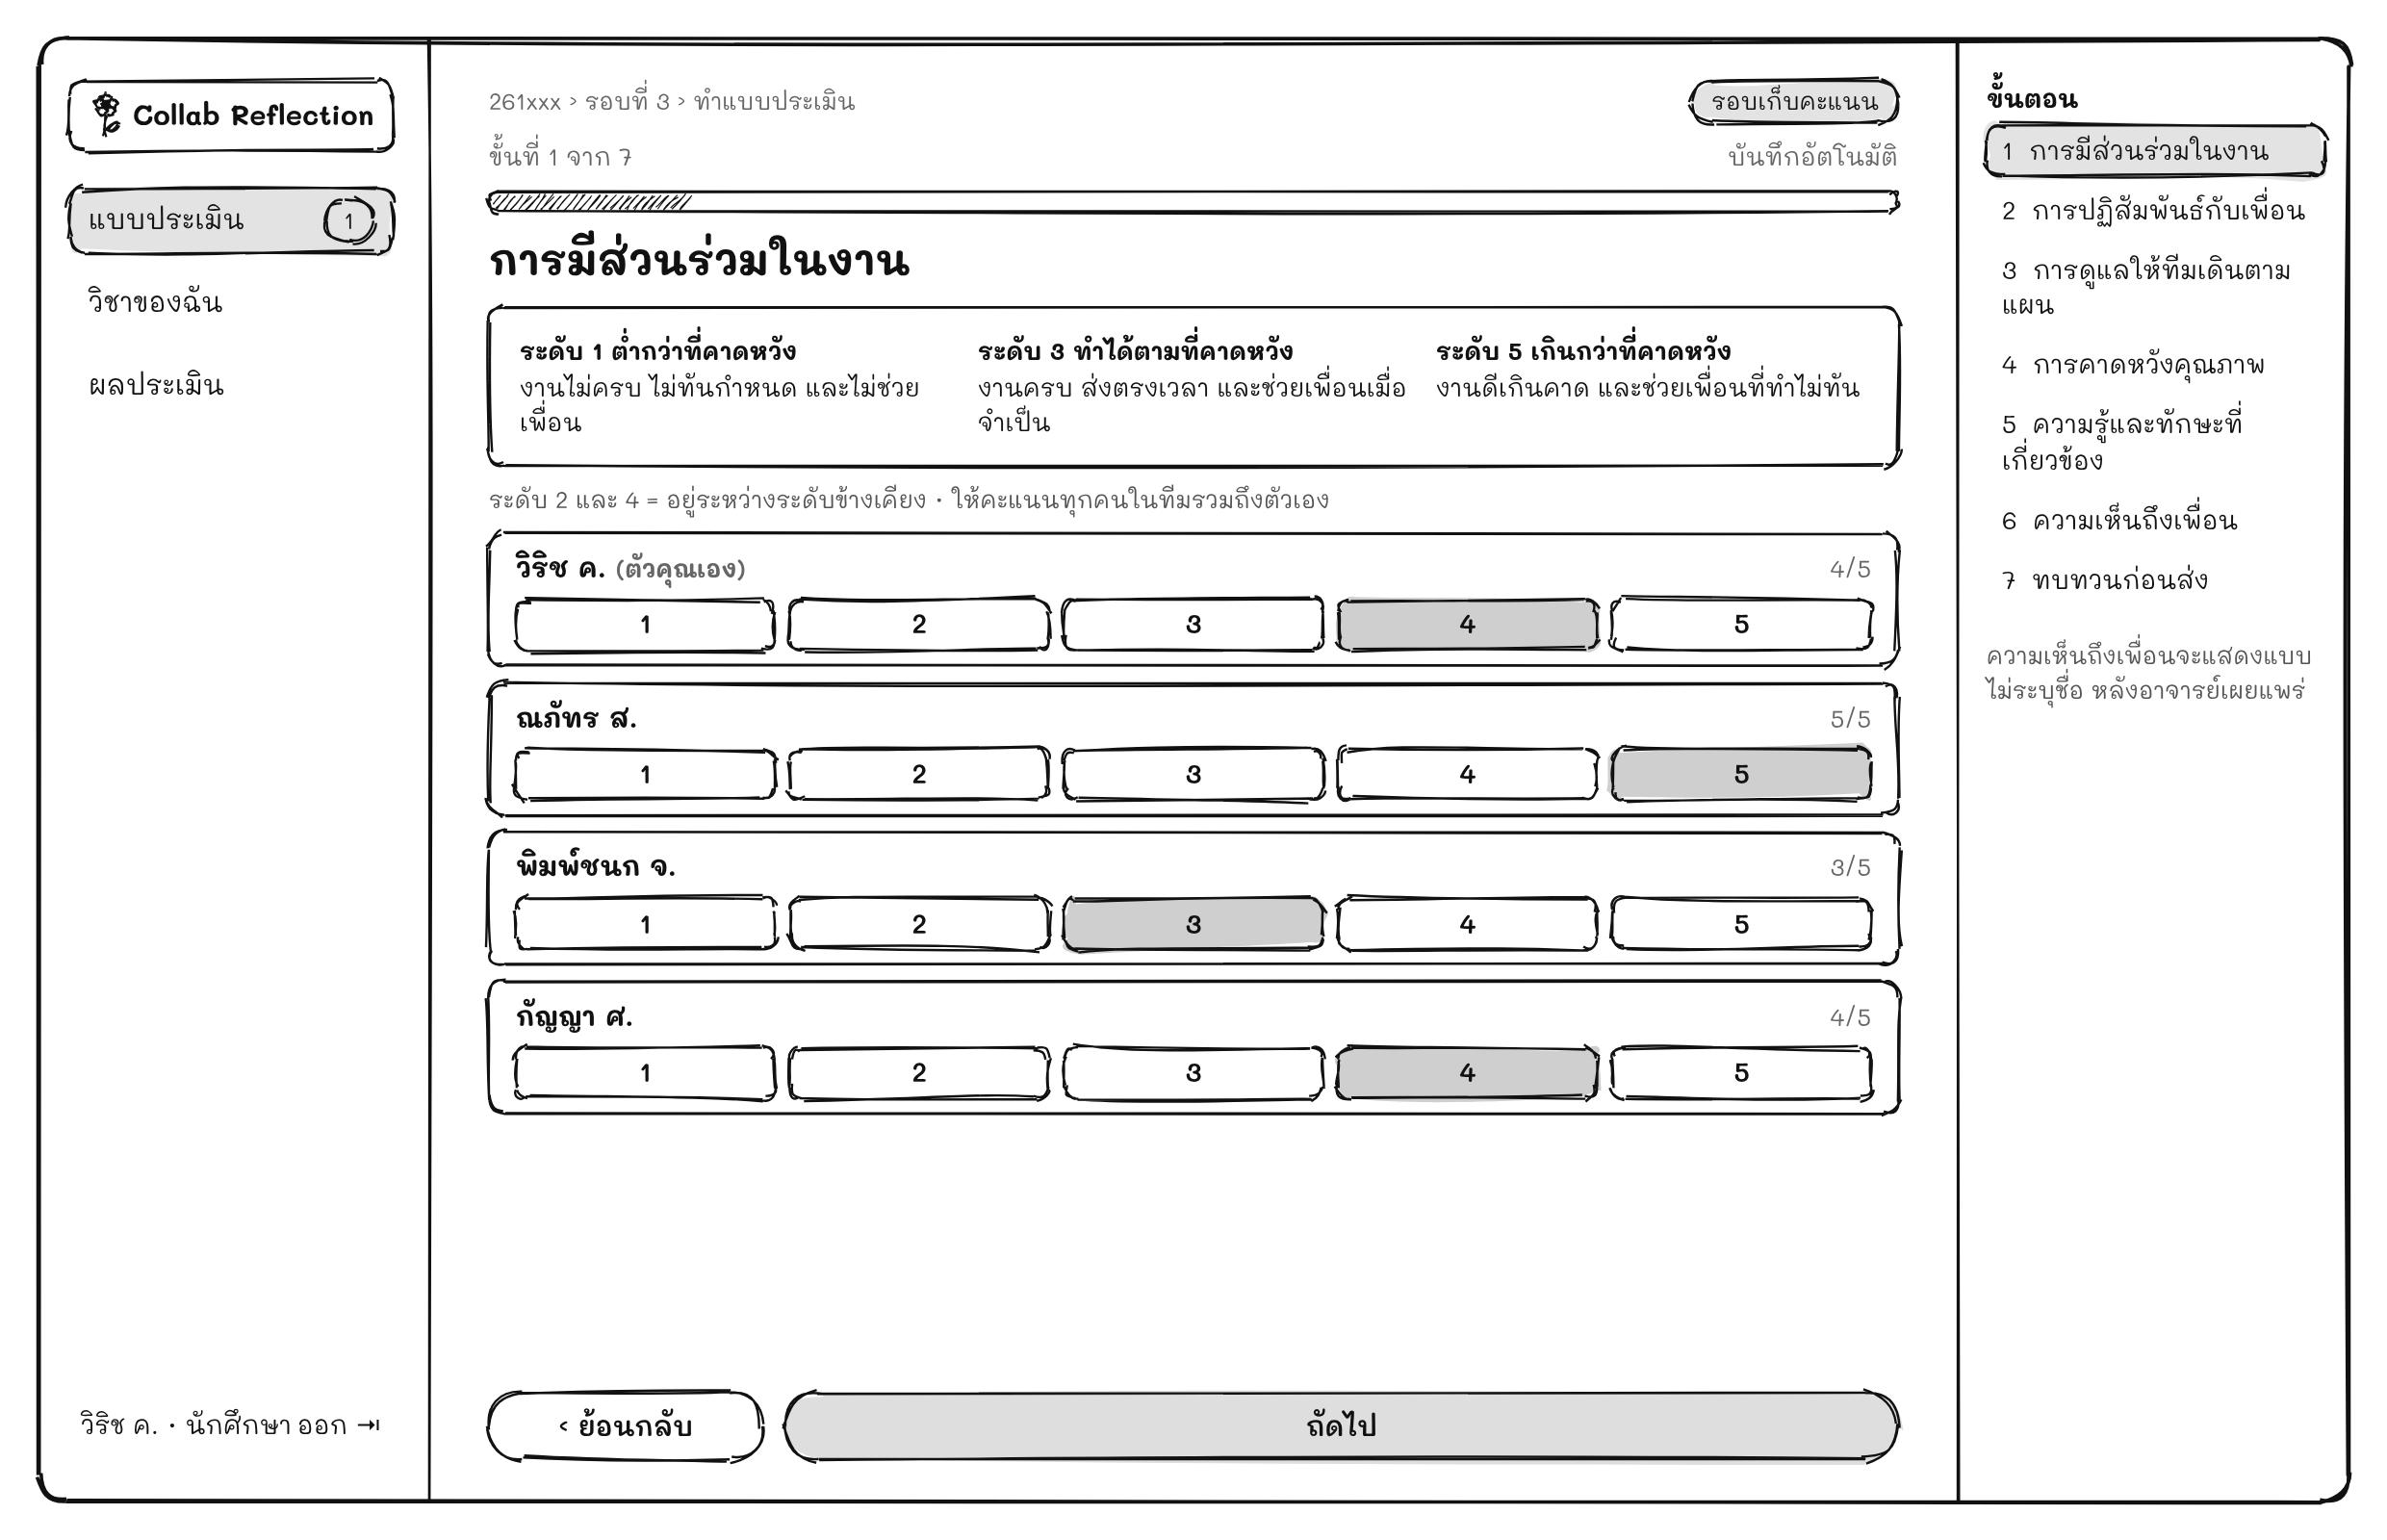
\includegraphics[width=0.85\textwidth]{figures/ch3/fig3-8-student-rating.png}}{\fbox{\parbox{0.8\textwidth}{\centering\vspace{2cm}[วางไฟล์ figures/ch3/fig3-8-student-rating.png]\vspace{2cm}}}}
\caption{หน้าให้คะแนนรายด้าน}\label{fig:ch3-8}
\end{figure}

ขั้นความเห็นถึงเพื่อนใช้แนวคิด ``ให้ดอกไม้ เติมปุ๋ย'' ดอกไม้คือสิ่งที่เพื่อนทำดีอยู่แล้วและควรได้รับคำชมเพื่อให้เติบโตต่อ ส่วนปุ๋ยเป็นสิ่งที่ช่วยให้เพื่อนเติบโตในงานถัดไป หน้าจอมีกล่องอธิบายพร้อมตัวอย่างการเขียน และภาพประกอบการเติบโตจากต้นอ่อนเป็นดอกไม้ ดังรูปที่~\ref{fig:ch3-9}

\begin{figure}[htbp]
\centering
\IfFileExists{figures/ch3/fig3-9-student-comments.png}{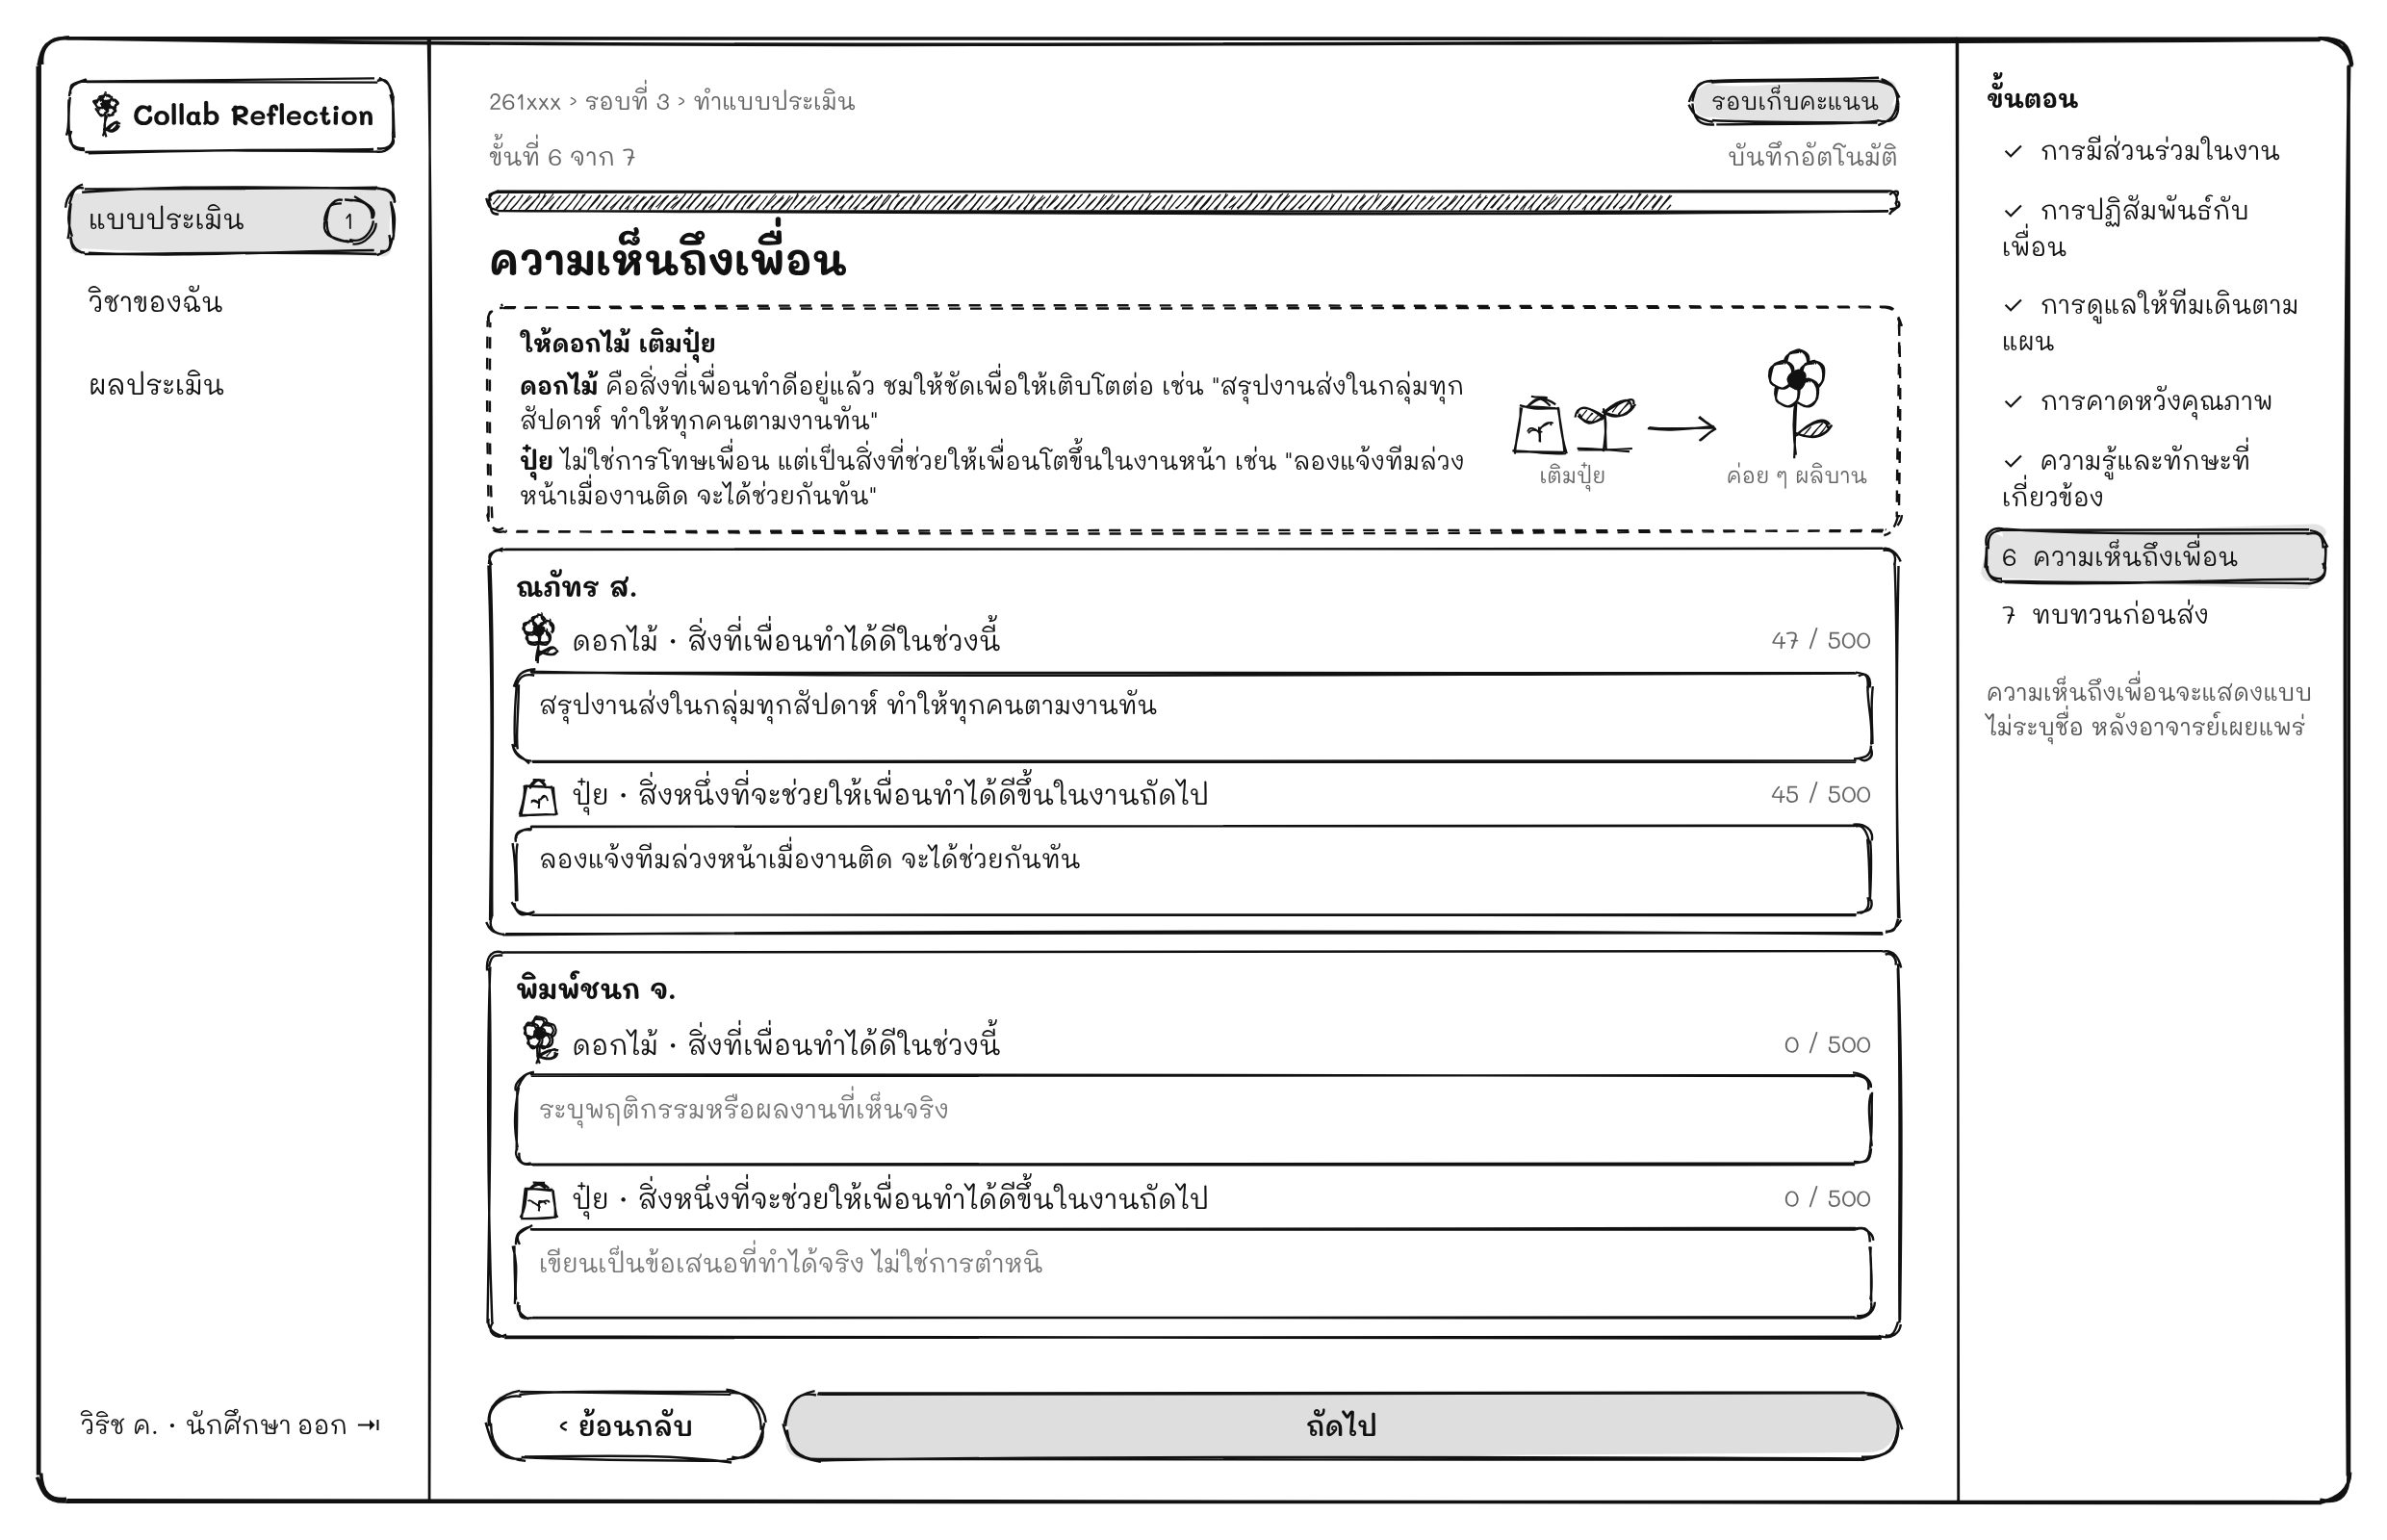
\includegraphics[width=0.85\textwidth]{figures/ch3/fig3-9-student-comments.png}}{\fbox{\parbox{0.8\textwidth}{\centering\vspace{2cm}[วางไฟล์ figures/ch3/fig3-9-student-comments.png]\vspace{2cm}}}}
\caption{หน้าเขียนความเห็นแบบดอกไม้และปุ๋ย}\label{fig:ch3-9}
\end{figure}

หน้าดูผลแสดงคะแนนรายด้านด้วยแผนภูมิเรดาร์ เปรียบเทียบค่าเฉลี่ยที่เพื่อนประเมินกับคะแนนที่ประเมินตนเอง แสดงดอกไม้และปุ๋ยที่ได้รับ ข้อเสนอแนะจากอาจารย์ และมีปุ่มขอความช่วยเหลือสำหรับนักศึกษาที่รู้สึกไม่สบายใจ ดังรูปที่~\ref{fig:ch3-10}

\begin{figure}[htbp]
\centering
\IfFileExists{figures/ch3/fig3-10-student-result.png}{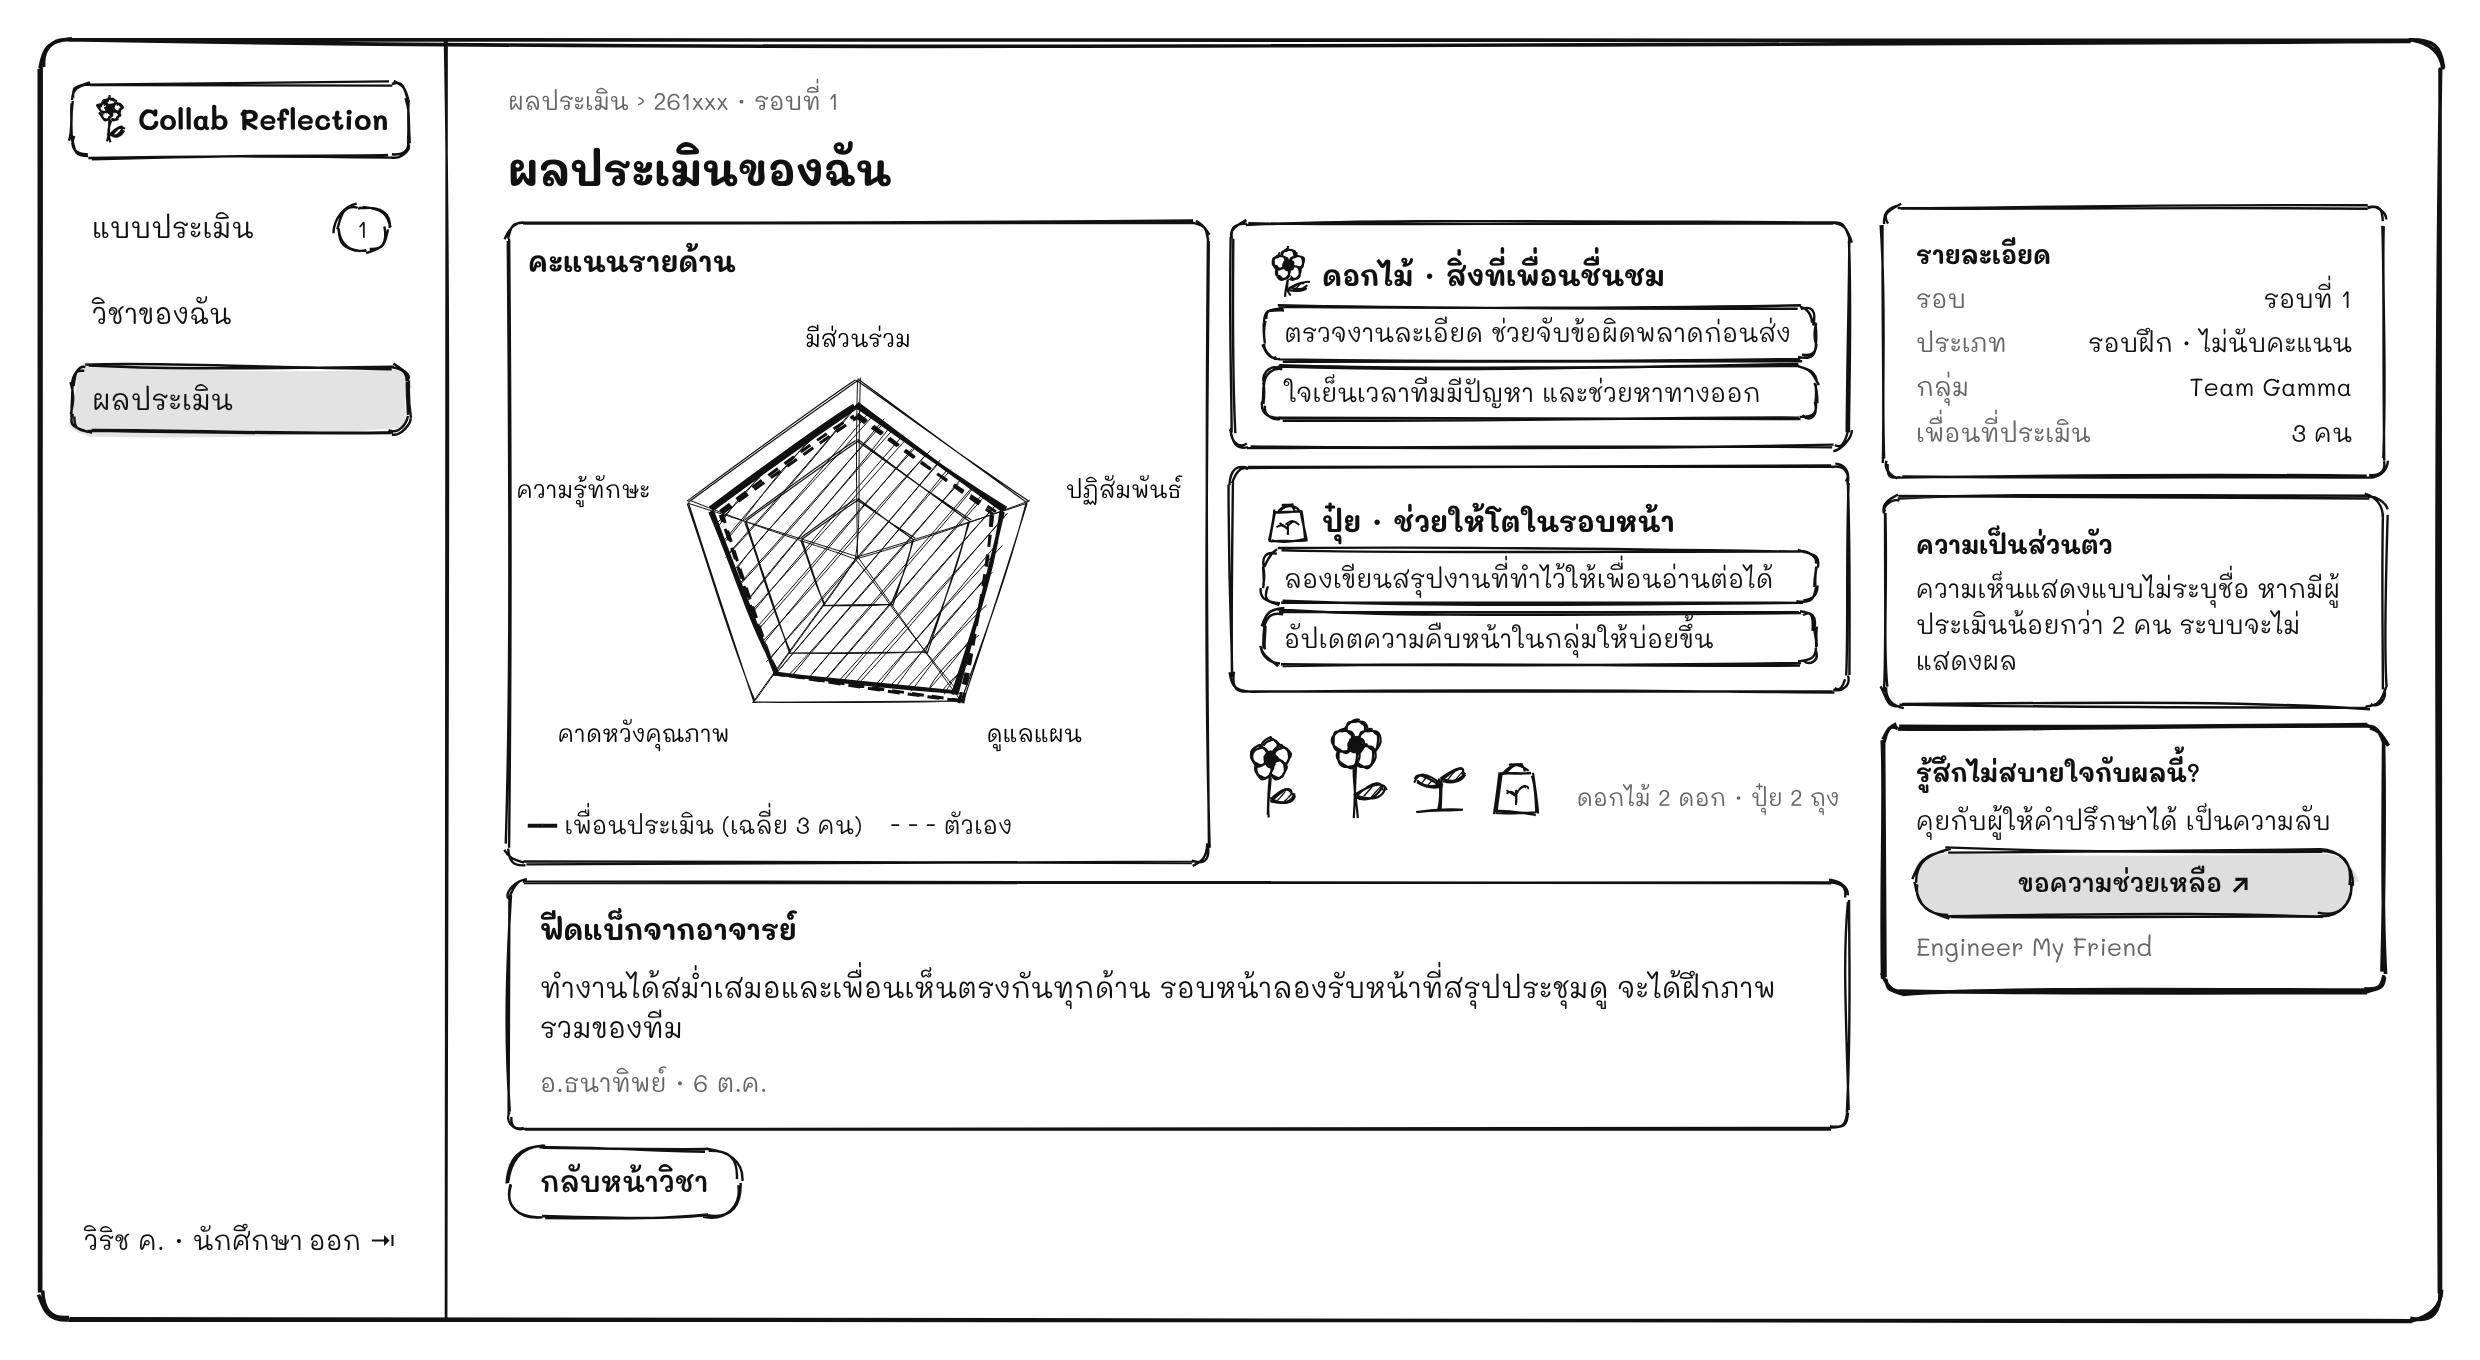
\includegraphics[width=\textwidth]{figures/ch3/fig3-10-student-result.png}}{\fbox{\parbox{0.8\textwidth}{\centering\vspace{2cm}[วางไฟล์ figures/ch3/fig3-10-student-result.png]\vspace{2cm}}}}
\caption{หน้าดูผลการประเมินของนักศึกษา}\label{fig:ch3-10}
\end{figure}

\subsection{หน้าจอฝั่งอาจารย์}\label{sec:3.8.3}

หน้าสมาชิกใช้นำเข้ารายชื่อนักศึกษาจากไฟล์ CSV จัดกลุ่ม และตรวจว่านักศึกษาคนใดยังไม่ยอมรับข้อตกลง PDPA ดังรูปที่~\ref{fig:ch3-11}

\begin{figure}[htbp]
\centering
\IfFileExists{figures/ch3/fig3-11-instructor-members.png}{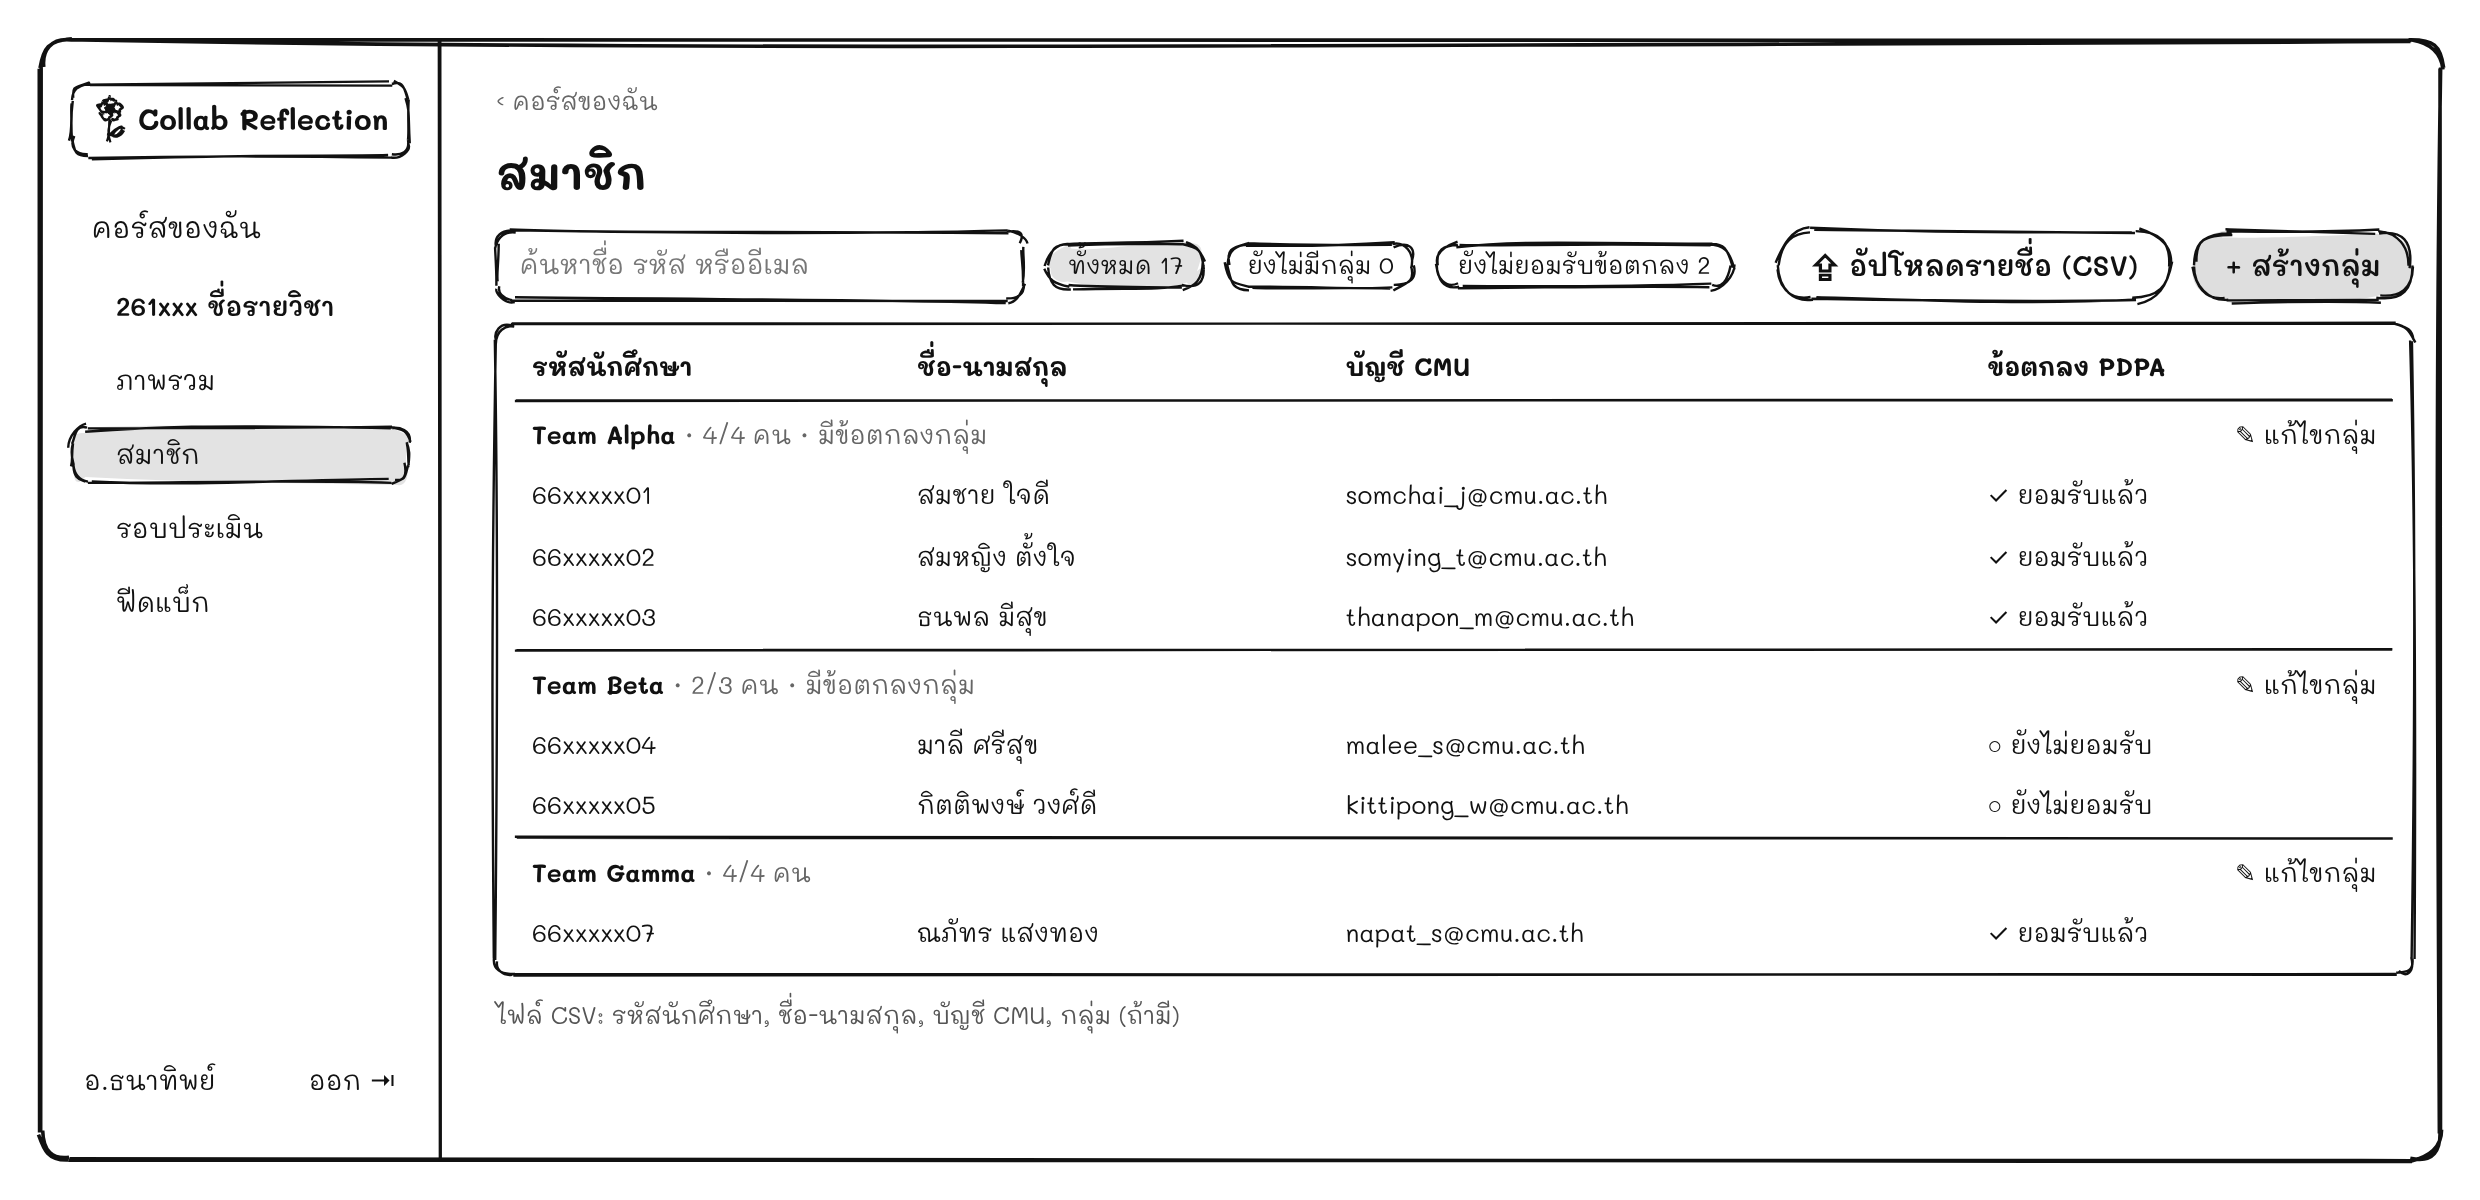
\includegraphics[width=\textwidth]{figures/ch3/fig3-11-instructor-members.png}}{\fbox{\parbox{0.8\textwidth}{\centering\vspace{2cm}[วางไฟล์ figures/ch3/fig3-11-instructor-members.png]\vspace{2cm}}}}
\caption{หน้าจัดการสมาชิกและกลุ่ม}\label{fig:ch3-11}
\end{figure}

หน้ารอบประเมินแสดงรอบทั้งหมดของรายวิชา เมื่อเพิ่มรอบใหม่ อาจารย์ต้องเลือกประเภทของรอบ (รอบฝึกหรือรอบเก็บคะแนน) และกำหนดช่วงเวลาเปิดปิด ดังรูปที่~\ref{fig:ch3-12}

\begin{figure}[htbp]
\centering
\IfFileExists{figures/ch3/fig3-12-instructor-rounds.png}{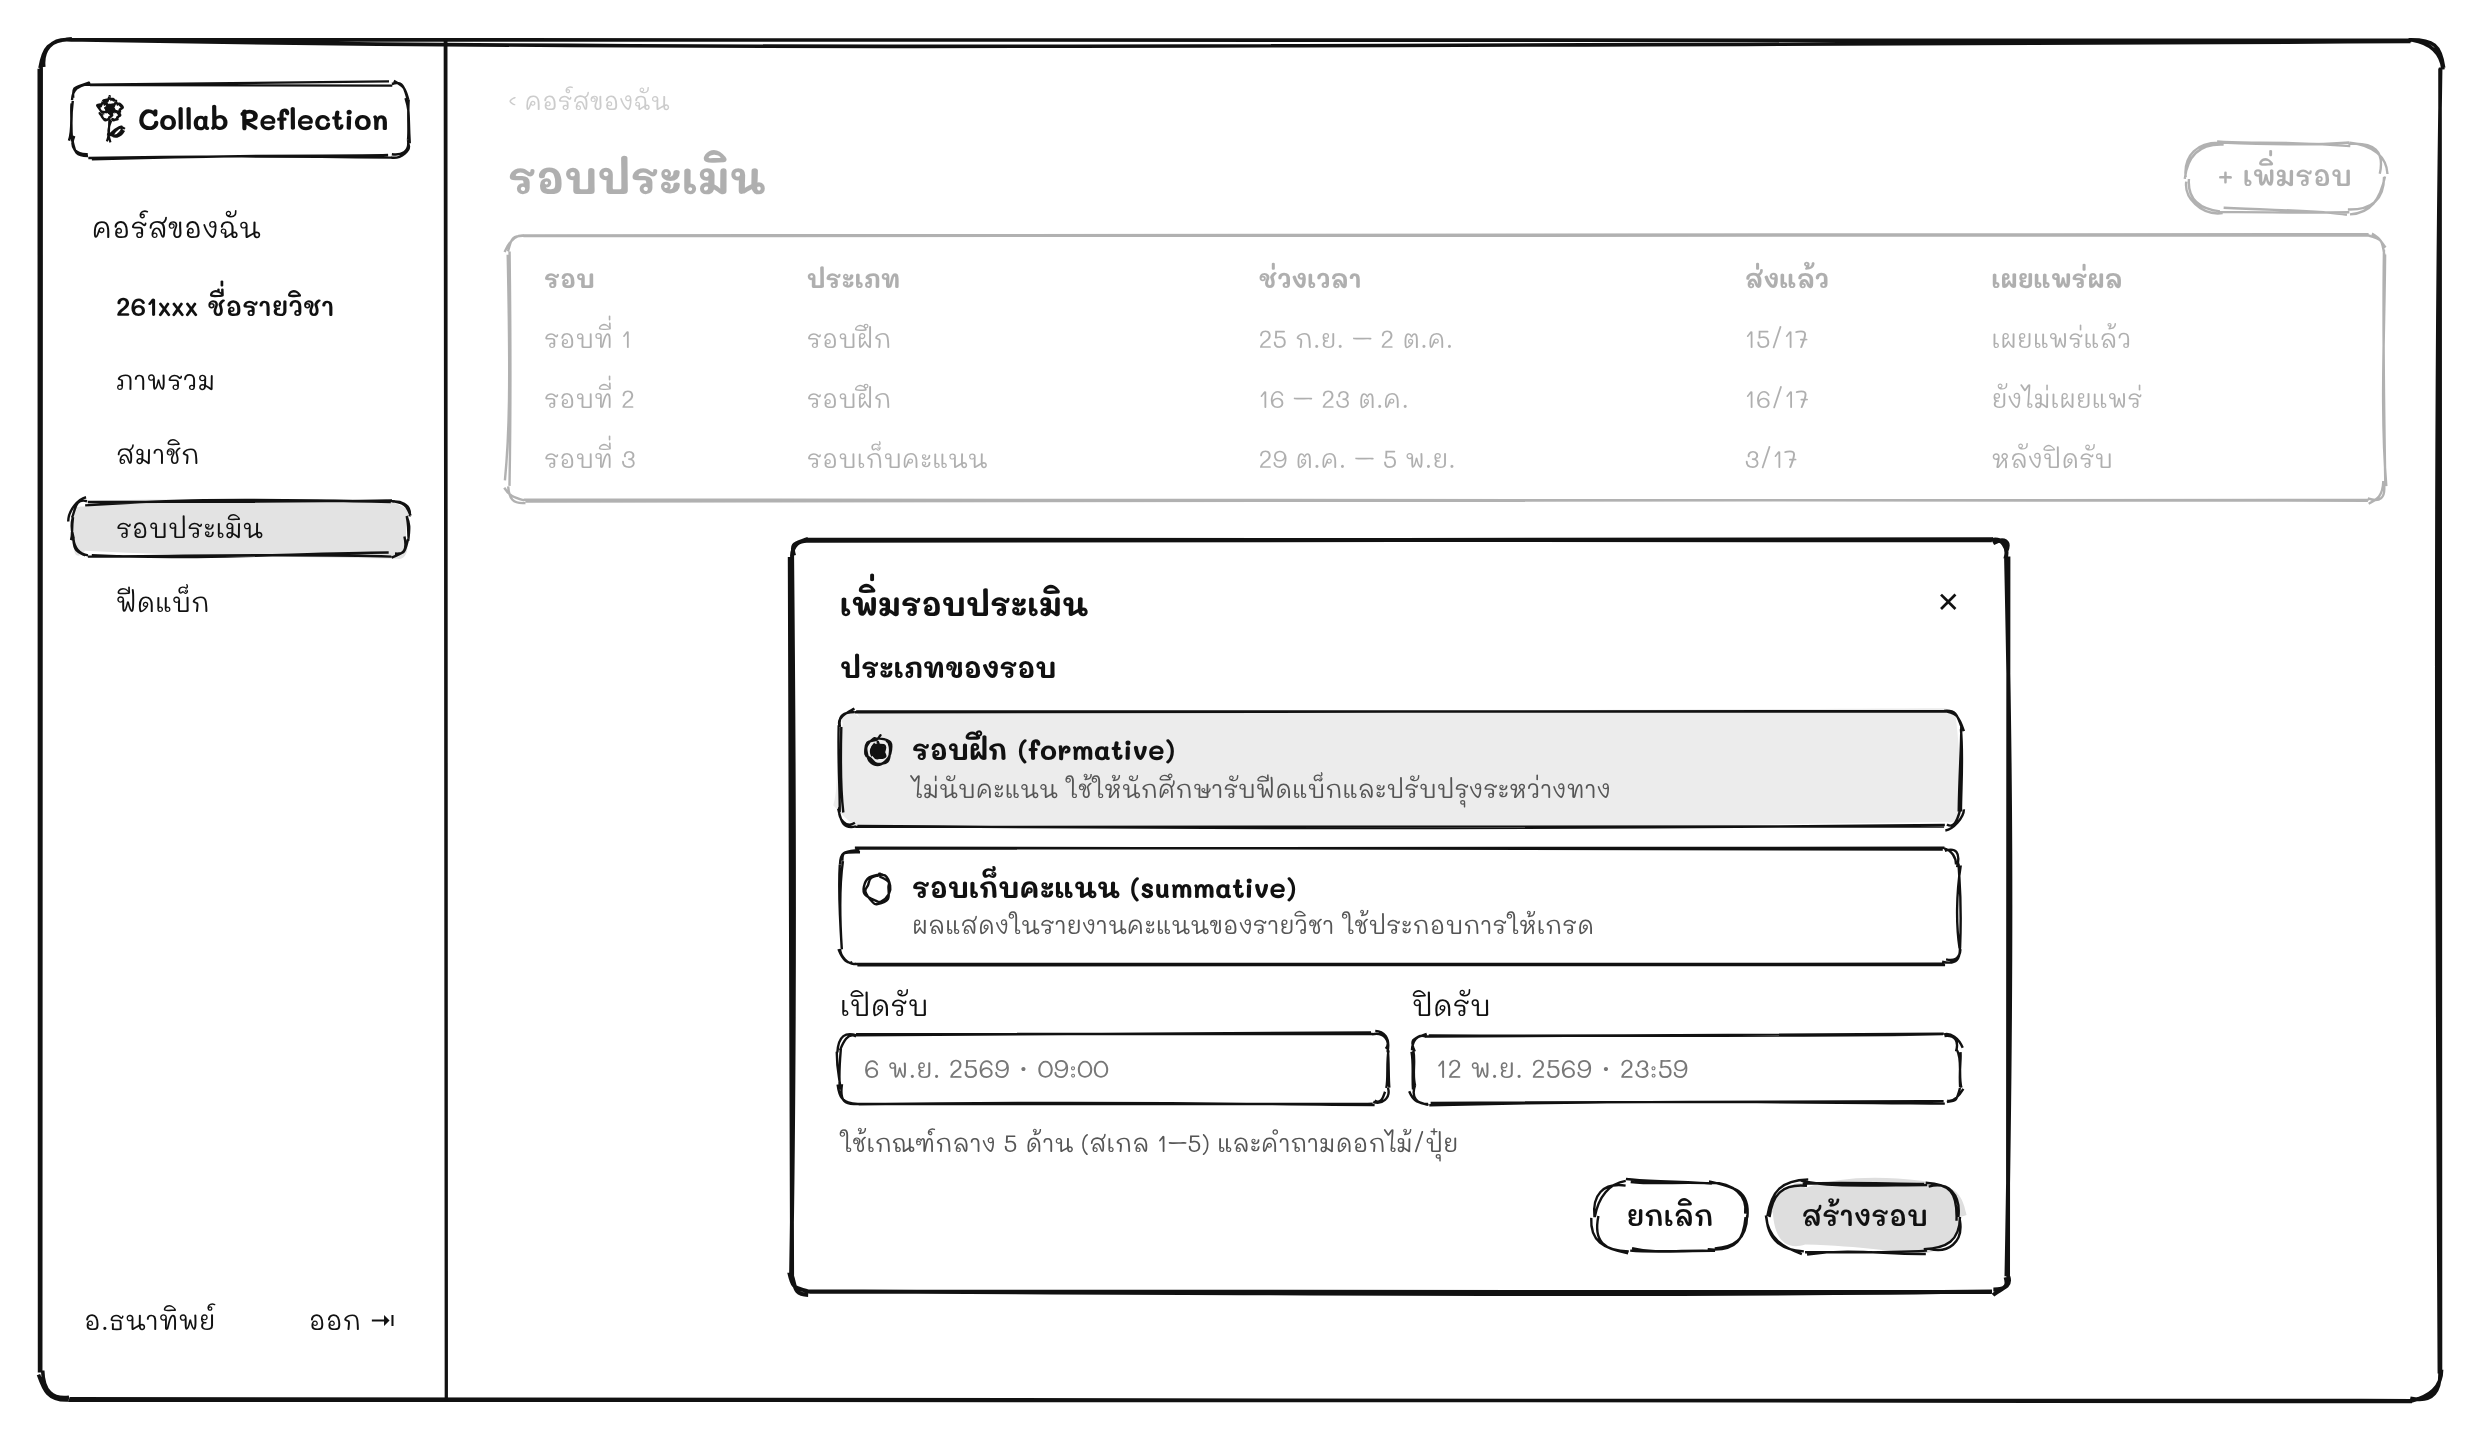
\includegraphics[width=\textwidth]{figures/ch3/fig3-12-instructor-rounds.png}}{\fbox{\parbox{0.8\textwidth}{\centering\vspace{2cm}[วางไฟล์ figures/ch3/fig3-12-instructor-rounds.png]\vspace{2cm}}}}
\caption{หน้าเพิ่มรอบประเมิน}\label{fig:ch3-12}
\end{figure}

แดชบอร์ดแสดงภาพรวมของรอบที่เลือก จำนวนผู้ส่ง แผนภาพเปรียบเทียบคะแนนที่ประเมินตนเองกับที่เพื่อนประเมิน และสัญญาณที่ควรดูของแต่ละทีม ดังรูปที่~\ref{fig:ch3-13}

\begin{figure}[htbp]
\centering
\IfFileExists{figures/ch3/fig3-13-instructor-overview.png}{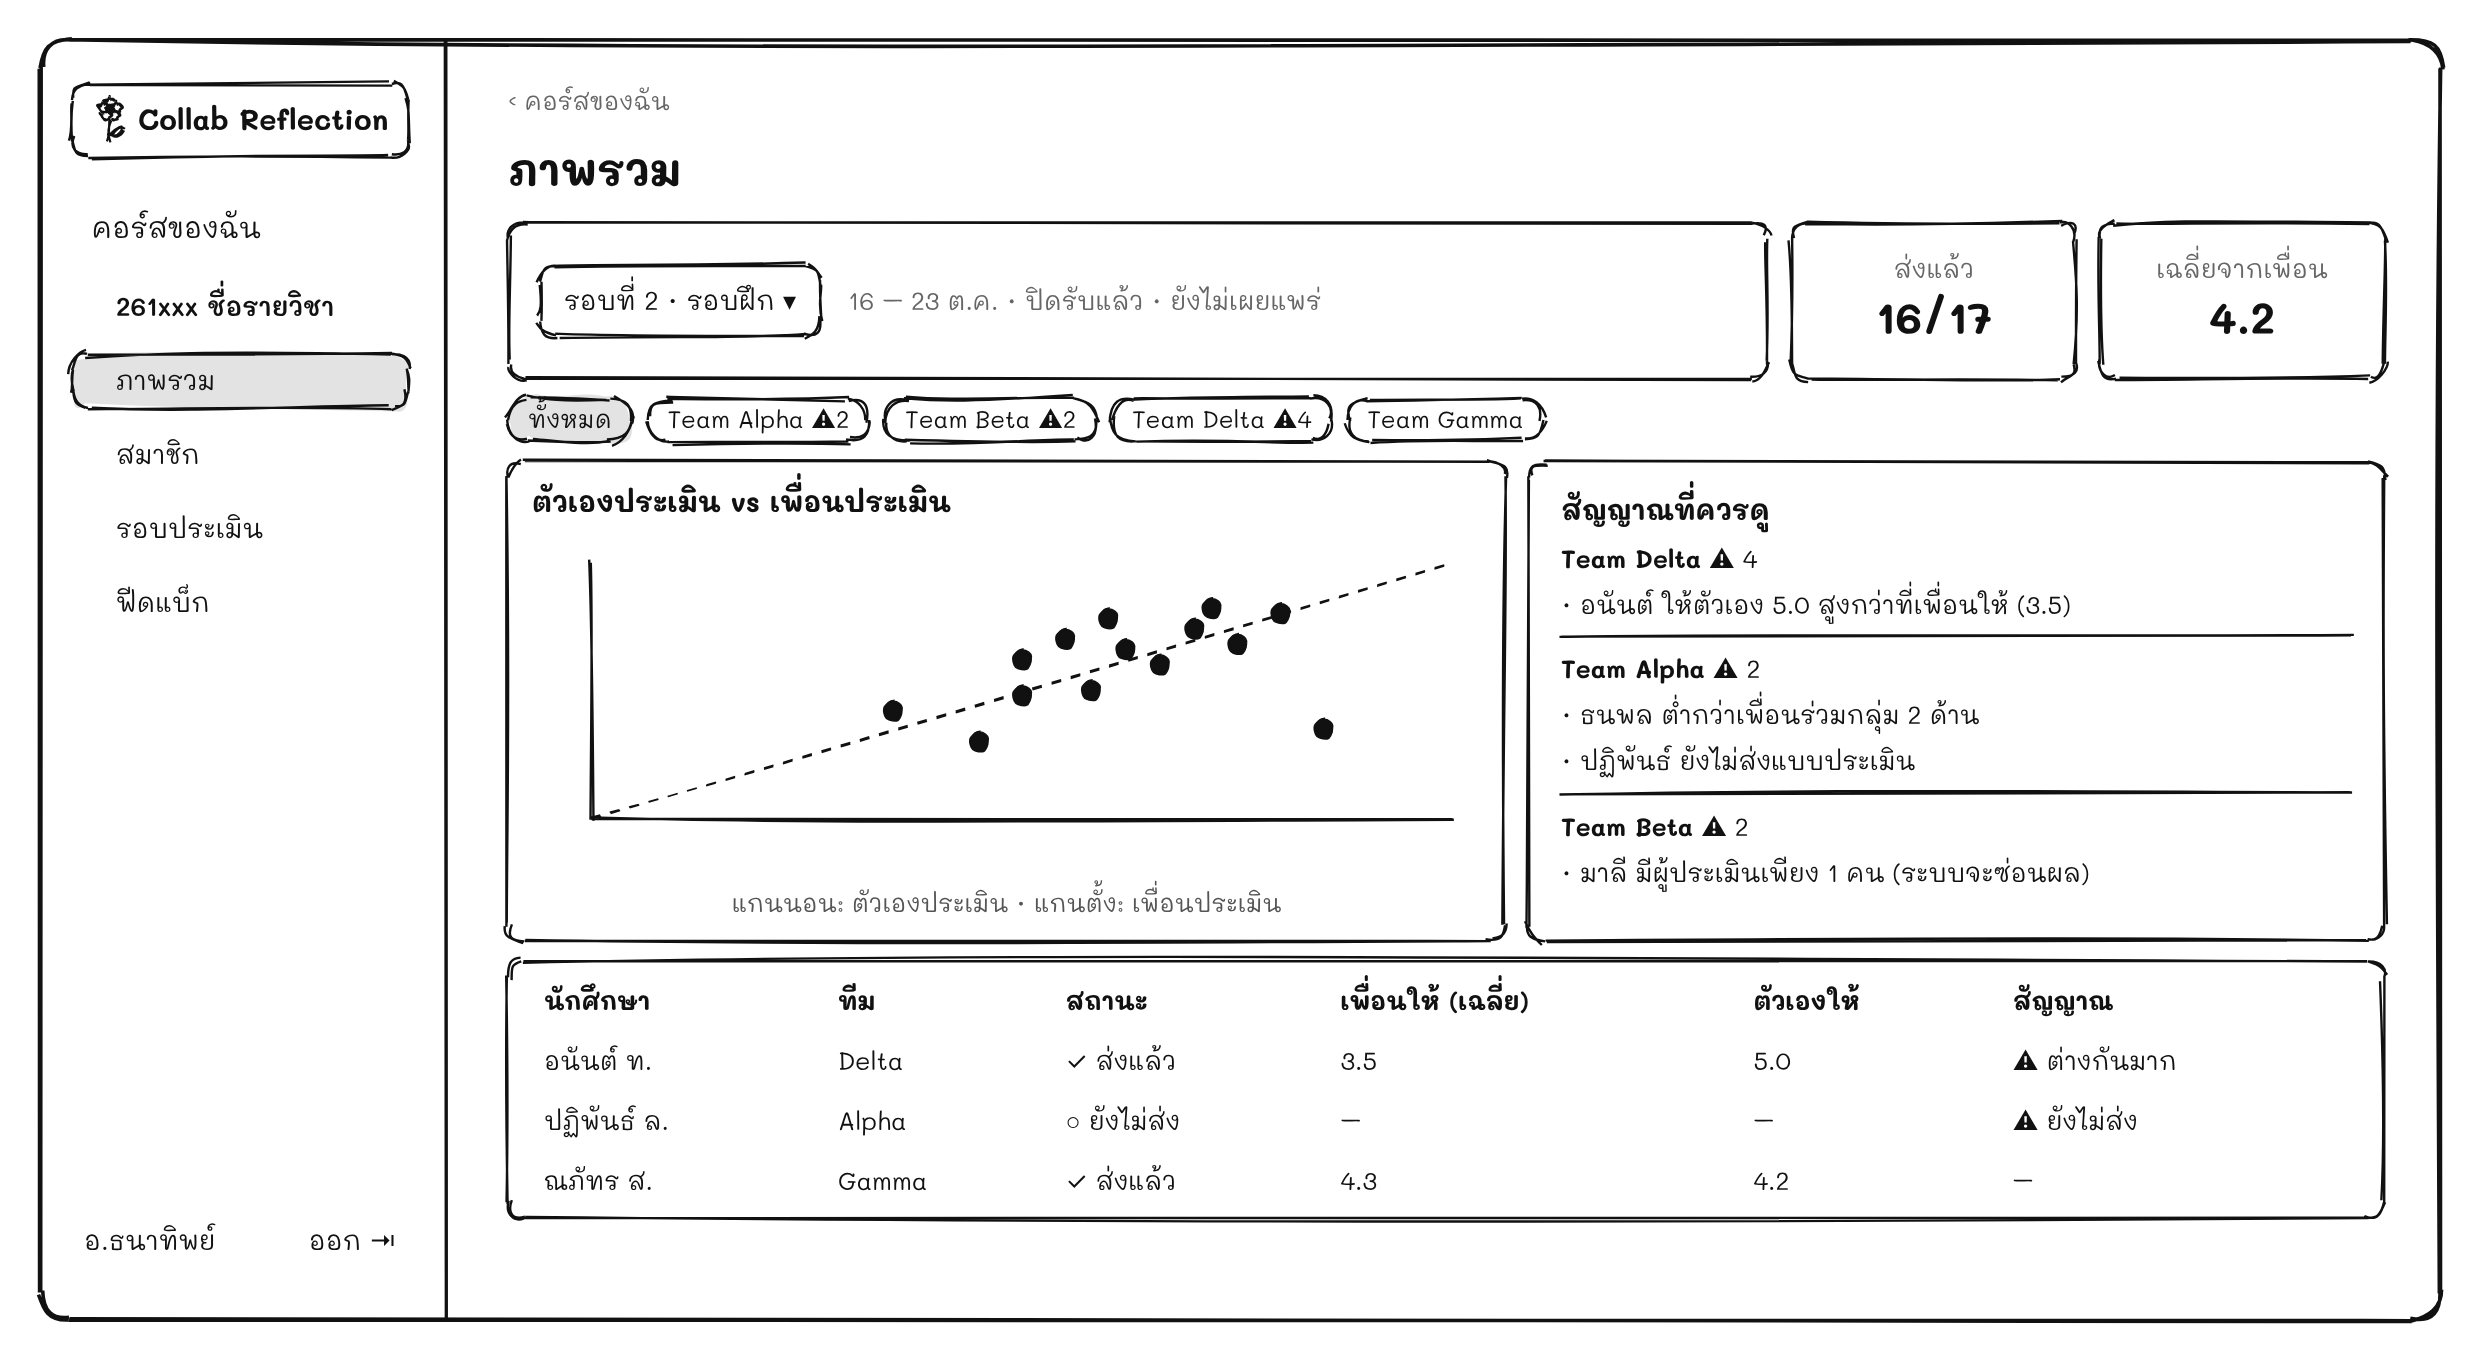
\includegraphics[width=\textwidth]{figures/ch3/fig3-13-instructor-overview.png}}{\fbox{\parbox{0.8\textwidth}{\centering\vspace{2cm}[วางไฟล์ figures/ch3/fig3-13-instructor-overview.png]\vspace{2cm}}}}
\caption{แดชบอร์ดของอาจารย์}\label{fig:ch3-13}
\end{figure}

หน้าภาพรวมแสดงผลของนักศึกษาทีละคน ให้อาจารย์อ่านดอกไม้และปุ๋ยจากเพื่อน เลือกว่านักศึกษาจะเห็นความเห็นของเพื่อนตามจริงหรือเฉพาะข้อสรุปของอาจารย์ เขียนข้อเสนอแนะ และกดเผยแพร่ผลของทั้งรอบ ดังรูปที่~\ref{fig:ch3-14}

\begin{figure}[htbp]
\centering
\IfFileExists{figures/ch3/fig3-14-instructor-feedback.png}{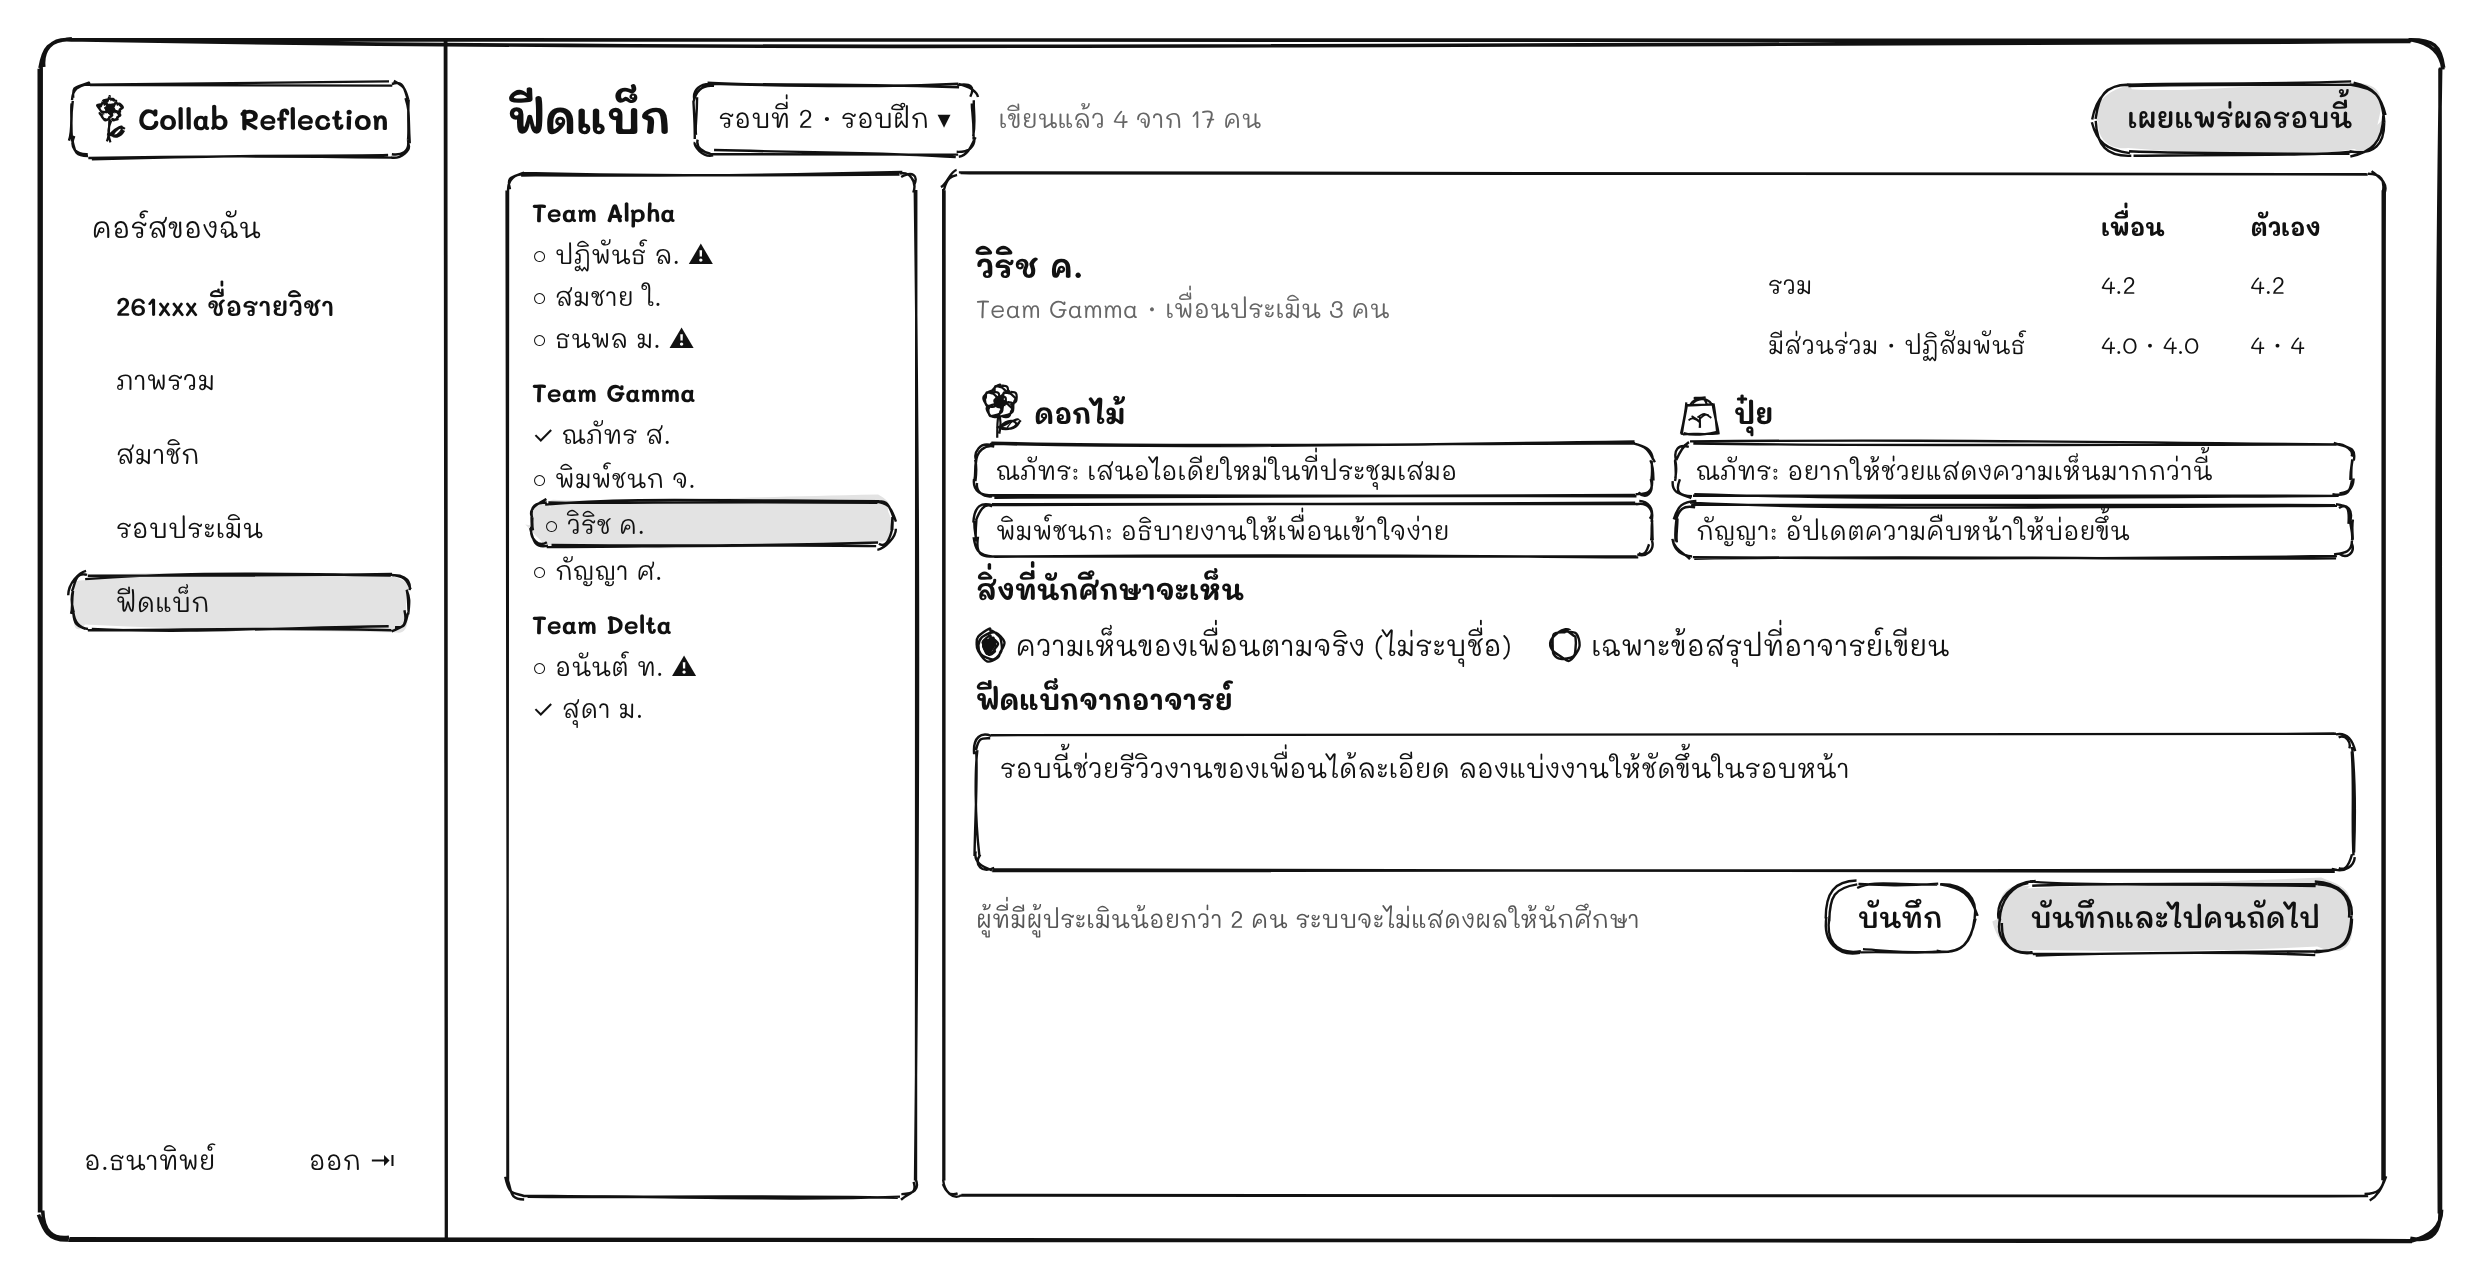
\includegraphics[width=\textwidth]{figures/ch3/fig3-14-instructor-feedback.png}}{\fbox{\parbox{0.8\textwidth}{\centering\vspace{2cm}[วางไฟล์ figures/ch3/fig3-14-instructor-feedback.png]\vspace{2cm}}}}
\caption{หน้าตรวจทานและเผยแพร่ผล}\label{fig:ch3-14}
\end{figure}

\section{ความปลอดภัยและการคุ้มครองข้อมูลส่วนบุคคล}\label{sec:3.9}

\subsection{ความปลอดภัยของระบบ}\label{sec:3.9.1}

\begin{itemize}
  \item เข้าสู่ระบบด้วยบัญชี CMU เท่านั้น และระบบไม่เก็บรหัสผ่าน
  \item ตรวจสิทธิ์ตามบทบาทในทุก API และบังคับกฎการปกปิดตัวตนที่ฝั่งเซิร์ฟเวอร์
  \item เข้ารหัสการสื่อสารด้วย HTTPS และใช้คุกกี้เซสชันแบบ HttpOnly และ Secure
  \item ตรวจสอบข้อมูลขาเข้าทุกครั้ง และใช้ ORM ที่สร้างคำสั่ง SQL แบบมีพารามิเตอร์ เพื่อป้องกัน SQL injection
  \item แบบประเมินที่ส่งแล้วแก้ไขไม่ได้ เพื่อป้องกันการเปลี่ยนคะแนนย้อนหลัง
\end{itemize}

\subsection{การคุ้มครองข้อมูลส่วนบุคคล}\label{sec:3.9.2}

ระบบออกแบบตามหลักของพระราชบัญญัติคุ้มครองข้อมูลส่วนบุคคล พ.ศ. 2562~\cite{pdpa2562} ได้แก่ เก็บข้อมูลเท่าที่จำเป็นต่อการประเมินงานกลุ่มเท่านั้น แจ้งก่อนใช้ว่าเก็บข้อมูลอะไร ใครเห็น และเก็บนานเท่าใด และให้เจ้าของข้อมูลใช้สิทธิ์ขอดู แก้ไข หรือลบข้อมูลได้

เพื่อไม่ให้นักศึกษาที่ไม่ยินยอมบางเรื่องต้องหลุดออกจากระบบจนเก็บคะแนนไม่ได้ ข้อตกลงจึงแบ่งเป็นส่วนจำเป็นและส่วนทางเลือก ดังตารางที่~\ref{tab:ch3-9} ทั้งนี้ คณะผู้จัดทำจะยืนยันระยะเวลาเก็บข้อมูลและฐานทางกฎหมายของการประมวลผลส่วนจำเป็นกับหน่วยงานที่ดูแลการคุ้มครองข้อมูลส่วนบุคคลของมหาวิทยาลัยก่อนใช้งานจริง

\begin{xltabular}{\textwidth}{|P{0.14\textwidth}|Y|Y|}
\caption{การแบ่งข้อตกลงการใช้ข้อมูลส่วนบุคคล}\label{tab:ch3-9}\\
\hline \textbf{ส่วน} & \textbf{ข้อมูลและการใช้งาน} & \textbf{หากไม่ยินยอม} \\ \hline
\endfirsthead
\multicolumn{3}{r}{\small (ต่อ)}\\ \hline \textbf{ส่วน} & \textbf{ข้อมูลและการใช้งาน} & \textbf{หากไม่ยินยอม} \\ \hline
\endhead
ส่วนจำเป็น & ข้อมูลบัญชี CMU รายวิชาและกลุ่มที่สังกัด คะแนนและความเห็นที่ใช้ในการประเมินของรายวิชา & ต้องรับทราบจึงจะใช้ระบบได้ เพราะเป็นข้อมูลขั้นต่ำของการประเมิน \\ \hline
ส่วนทางเลือก 1 & ส่งข้อความที่เขียนให้ปัญญาประดิษฐ์ (AI) ประมวลผล (เฟสที่ 2) & ใช้ระบบและได้คะแนนตามปกติ แต่ข้อความของผู้นั้นจะไม่ถูกส่งให้ปัญญาประดิษฐ์ (AI) \\ \hline
ส่วนทางเลือก 2 & นำข้อมูลแบบไม่ระบุตัวตนไปใช้พัฒนาระบบและในงานวิจัย & ใช้ระบบและได้คะแนนตามปกติ แต่ข้อมูลของผู้นั้นจะไม่ถูกนำไปใช้ \\ \hline
\end{xltabular}

\subsection{การดูแลความรู้สึกของผู้ใช้}\label{sec:3.9.3}

ข้อเสนอแนะจากเพื่อนอาจกระทบความรู้สึกของผู้รับได้แม้ผ่านการกลั่นกรองแล้ว ระบบจึงลดโอกาสเกิดความคิดเห็นที่ทำร้ายจิตใจตั้งแต่ต้นทาง ด้วยคำถามแบบดอกไม้และปุ๋ย คำแนะนำการเขียน และการตรวจทานของอาจารย์ก่อนเผยแพร่ และที่หน้าดูผลมีปุ่มขอความช่วยเหลือที่เชื่อมไปยังช่องทางให้คำปรึกษา เช่น โครงการ Entaneer Mind Friend สำหรับนักศึกษาที่รู้สึกไม่สบายใจ

\section{แผนการประเมินระบบและตัวชี้วัดความสำเร็จ}\label{sec:3.10}

การประเมินระบบอยู่ในระยะที่ 4 ของการดำเนินงาน แบ่งเป็นการตรวจสอบว่าระบบทำงานถูกต้องตามที่ออกแบบ (verification) และการยืนยันว่าระบบแก้ปัญหาของผู้ใช้ได้จริง (validation)

\subsection{การตรวจสอบความถูกต้องของระบบ}\label{sec:3.10.1}

\begin{itemize}
  \item Unit test ด้วย Vitest สำหรับตรรกะสำคัญ เช่น การคำนวณค่าเฉลี่ยรายด้าน เงื่อนไขซ่อนผลเมื่อผู้ประเมินไม่ถึง 2 คน และเงื่อนไขสัญญาณเตือน
  \item Integration test ของ API ทุกเส้นทาง รวมถึงทดสอบว่านักศึกษาเรียกดูข้อมูลที่ตนไม่มีสิทธิ์ไม่ได้
  \item End-to-end test ด้วย Cypress สำหรับขั้นตอนหลัก ได้แก่ นักศึกษาส่งแบบประเมิน และอาจารย์ตรวจทานและเผยแพร่ผล
  \item ทดสอบโหลดด้วยจำนวนผู้ใช้เทียบเท่าหนึ่งรายวิชา
  \item ส่วน AI (เฟสที่ 2): วัดความสอดคล้องระหว่างผลการตรวจโทนของโมเดลกับการติดป้ายกำกับโดยคน บนชุดข้อความภาษาไทยตัวอย่าง
\end{itemize}

\subsection{การนำร่องใช้งานจริง}\label{sec:3.10.2}

คณะผู้จัดทำจะนำระบบไปทดลองใช้ในรายวิชาที่มีการทำงานกลุ่มระยะยาวของภาควิชาวิศวกรรมคอมพิวเตอร์อย่างน้อย 1 รายวิชา โดยมีรอบฝึกอย่างน้อย 1 รอบและรอบเก็บคะแนน 1 รอบ หลังใช้งานจะเก็บแบบสอบถาม System Usability Scale (SUS)~\cite{brooke1996sus} จากทั้งอาจารย์และนักศึกษา และสัมภาษณ์อาจารย์ผู้สอนเรื่องภาระงานและประโยชน์ที่ได้รับ เพื่อนำไปพัฒนาในระยะถัดไป

\subsection{ตัวชี้วัดความสำเร็จ}\label{sec:3.10.3}

ตัวชี้วัดความสำเร็จของโครงงานแสดงในตารางที่~\ref{tab:ch3-10}

\begin{xltabular}{\textwidth}{|P{0.14\textwidth}|P{0.2\textwidth}|Y|P{0.15\textwidth}|}
\caption{ตัวชี้วัดความสำเร็จของโครงงาน}\label{tab:ch3-10}\\
\hline \textbf{ด้าน} & \textbf{ตัวชี้วัด} & \textbf{เป้าหมาย} & \textbf{วิธีวัด} \\ \hline
\endfirsthead
\multicolumn{4}{r}{\small (ต่อ)}\\ \hline \textbf{ด้าน} & \textbf{ตัวชี้วัด} & \textbf{เป้าหมาย} & \textbf{วิธีวัด} \\ \hline
\endhead
ความถูกต้องของระบบ & กรณีทดสอบของฟีเจอร์ระยะที่ 1 & ผ่านทั้งหมด & Vitest และ Cypress \\ \hline
การใช้งานจริง & จำนวนรายวิชานำร่อง & อย่างน้อย 1 รายวิชา และ 2 รอบประเมิน & บันทึกการใช้งานในระบบ \\ \hline
การรองรับผู้ใช้ & จำนวนผู้ใช้ที่ใช้งานพร้อมกันได้ & ประมาณ 90 คนต่อรายวิชา ตามสัดส่วนนักศึกษาต่ออาจารย์ในรายวิชาเป้าหมาย & ทดสอบโหลด \\ \hline
การมีส่วนร่วม & อัตราการส่งแบบประเมินต่อรอบ & อย่างน้อยร้อยละ 80 & ข้อมูลในระบบ \\ \hline
ความง่ายในการใช้งาน & คะแนน SUS & อย่างน้อย 68 คะแนน ซึ่งเป็นค่าเฉลี่ยอ้างอิงทั่วไป~\cite{sauro2011sus} ทั้งฝั่งอาจารย์และนักศึกษา & แบบสอบถาม SUS \\ \hline
ภาระงานของอาจารย์ & เวลาที่ใช้ตรวจทานและเผยแพร่ผลต่อหนึ่งกลุ่ม & น้อยกว่าวิธีเดิมที่อาจารย์ใช้อยู่ & จับเวลาและสัมภาษณ์อาจารย์ \\ \hline
คุณภาพฟีดแบ็ก & สัดส่วนความเห็นที่ระบุพฤติกรรมและเสนอสิ่งที่ทำได้จริง & รอบเก็บคะแนนสูงกว่ารอบฝึกรอบแรก & จัดหมวดความเห็นโดยผู้ประเมิน 2 คน \\ \hline
\end{xltabular}

